% !TEX program = pdflatex
\documentclass[conference,10pt]{IEEEtran}

% ── Packages ──
\usepackage{amsmath,amssymb,amsthm}
\usepackage{graphicx}
\usepackage{booktabs}
\usepackage{hyperref}
\usepackage{xcolor}
\usepackage{enumitem}
\usepackage{float}
\usepackage{caption}
\usepackage{url}
\usepackage{cite}
\usepackage{microtype}

% Use CM typewriter (avoids missing Courier font)
\renewcommand{\ttdefault}{cmtt}

\hypersetup{
  colorlinks=true,
  linkcolor=blue!70!black,
  citecolor=green!50!black,
  urlcolor=blue!60!black,
}

% ── Figure path ──
\graphicspath{{../results/figures/}}

% ── Theorem env ──
\newtheorem{proposition}{Proposition}

% ── Compact lists ──
\setlist{nosep,leftmargin=1.5em}

% ══════════════════════════════════════════════════════════════════
\title{OpsSkill: Autonomous Operations Skill Learning\\for Cloud-Native Systems}

\author{
\IEEEauthorblockN{Anonymous}
\IEEEauthorblockA{\textit{Under Review}}
}

\begin{document}
\maketitle

% ================================================================
%  Abstract
% ================================================================
\begin{abstract}
As large language models (LLMs) demonstrate increasing capability in tool invocation and autonomous agents, leveraging them for automated operations in DevOps and SRE scenarios has become an important research direction.
However, existing methods mostly model operations tasks as free-form command generation or interactive tool-calling processes, lacking unified modeling of preconditions, action constraints, success criteria, rollback mechanisms, and risk boundaries, making it difficult to achieve safe, reliable, and reusable automated execution in real infrastructure environments.

This paper proposes \textbf{OpsSkill}, an autonomous operations skill learning framework for cloud-native systems.
OpsSkill automatically compiles task cards into structured skill representations containing preconditions, action sequences, hidden verifiers, rollback plans, and risk labels; during execution, it controls skill deployment through policy constraints and capability probing; during optimization, it continuously improves skills based on structured execution reports and failure signatures.
Unlike evaluations that rely solely on command return values, OpsSkill further designs a multi-signal hidden verification mechanism for real remote environments, combining object state, events, logs, and service health information to determine whether a skill has truly accomplished its operational objective.
The framework's core designs (Typed Skill IR, gated execution, hidden verification) are platform-agnostic and applicable to Kubernetes, OpenStack, AWS, and other cloud-native platforms.

We validate OpsSkill on a Kubernetes cluster (3 nodes, K8s v1.33.6) as a representative platform, injecting CPU stress, memory stress, and network delay faults via Chaos Mesh across 8 operations tasks.
We compare against direct command generation, ReAct-style agents, Reflexion-style optimization, and template retrieval as four baselines, and quantify each component's contribution through ablation studies.
OpsSkill achieves a 90\% composite score, outperforming direct command generation (25\%), ReAct (40\%), Reflexion (40\%), and template retrieval (25\%) by 50--65 percentage points, while maintaining zero unsafe action rate.
Ablation studies show that Typed Skill IR contributes 65\% of the score improvement, hidden verification contributes 30\%, and policy gating reduces the unsafe action rate from 12\% to 0\% at a cost of only 1\% in score.
\end{abstract}

\begin{IEEEkeywords}
Autonomous operations, cloud-native systems, large language models, skill learning, safe execution
\end{IEEEkeywords}

% ================================================================
%  1  Introduction
% ================================================================
\section{Introduction}

With the widespread deployment of cloud-native systems and microservice architectures~\cite{burns2022kubernetes}, DevOps and SRE teams must continuously handle a large volume of repetitive yet high-risk operations tasks---fault diagnosis, configuration remediation, service recovery, scaling adjustments, and permission anomaly handling~\cite{beyer2016sre}.
These tasks typically rely on operators' comprehensive understanding of system state, toolchains, failure modes, and organizational constraints, exhibiting pronounced state dependency, environment heterogeneity, and execution risk.
Ghosh et al.~\cite{ghosh2022incidents} show through an empirical study of Microsoft Teams' large-scale cloud services that over 60\% of high-severity incidents involve multi-step diagnosis and remediation workflows, making automation imperative.
Recent advances in LLM reasoning~\cite{wei2022chain}, code generation, and tool calling~\cite{yao2023react} make it attractive to build autonomous agents that can assist or partially automate these tasks~\cite{cheng2023aiops}.

However, existing methods remain far from truly usable autonomous operations.
On one hand, many approaches simplify operations tasks into free-form command generation or interactive tool-calling~\cite{roy2024rca_agents}, ignoring that operations actions are heavily constrained and potentially costly.
For real production or pre-production environments, an incorrect command sequence may not only cause task failure but also lead to cross-scope impacts, service disruptions, or even irreversible data corruption~\cite{ruan2023toolemu}.
On the other hand, existing evaluations typically rely on visible command return codes or single check items to determine task completion~\cite{ye2024toolsword}, but in real systems, ``command success'' does not equate to ``service recovery.''
For example, a Pod being successfully restarted does not mean the dependency chain has recovered; a Deployment rollout completion does not mean the user-facing error rate has decreased.
Therefore, autonomous operations systems need not only to ``call tools'' but also to possess capabilities for safe execution, hidden verification, and post-failure optimization.

To address these challenges, we propose \textbf{OpsSkill}, an autonomous operations skill learning framework for cloud-native systems.
OpsSkill's core idea is to elevate operations tasks from one-shot command generation to structured skill learning.
The framework's core designs (Typed Skill IR, gated execution, hidden verification, failure-driven optimization) are platform-agnostic, applicable to Kubernetes, OpenStack, AWS, and other cloud-native platforms.
Specifically, we compile a task into a typed skill representation with preconditions, action sequences, success criteria, rollback plans, and risk labels; at the execution layer, we design policy-constrained gated execution with capability probing; at the evaluation layer, we introduce multi-signal hidden verifiers combining object state, events, logs, and service health to determine true task completion; at the optimization layer, we use structured execution reports and failure signatures~\cite{shinn2023reflexion} to continuously improve skill quality.

\noindent\textbf{Contributions:}
\begin{enumerate}
  \item A \textbf{Typed Ops Skill IR} that compiles task cards into structured skill objects with preconditions, actions, success criteria, rollback plans, and risk labels.
  \item A \textbf{policy-gated execution framework} with adaptive risk weighting that quantifies and bounds blast radius before execution, with a formal safety guarantee (Proposition~1).
  \item A \textbf{hidden multi-signal verification mechanism} combining visible and hidden checks to detect false positives.
  \item A \textbf{structured failure-driven optimization mechanism} that extracts failure signatures and maps them to deterministic IR edits, with a monotonic convergence guarantee (Proposition~2).
  \item Systematic evaluation on a real Kubernetes cluster (as a representative cloud-native platform) with baseline comparisons, ablation studies, unified evaluation metrics, and weight sensitivity analysis to verify conclusion robustness.
\end{enumerate}

% ================================================================
%  2  Related Work
% ================================================================
\section{Related Work}

Existing research most relevant to OpsSkill falls into four categories: AIOps and incident knowledge mining, microservice diagnosis and root cause localization, runbook automation, and agent tool-calling evaluation and safety governance.

\textbf{AIOps and Incident Knowledge Mining.}
The first category focuses on extracting structured knowledge from real cloud service incidents and operations investigations.
Cheng et al.~\cite{cheng2023aiops} provide a comprehensive AIOps survey, organizing techniques into anomaly detection, root cause analysis (RCA), incident triage, and automated remediation.
DeCaf~\cite{bansal2020decaf} models performance issue diagnosis and triage in large-scale cloud services as a continuous pipeline, automatically identifying fault root causes from KPI regression through machine learning and pattern mining, and has been deployed in multiple Microsoft cloud services.
Ghosh et al.~\cite{ghosh2022incidents} empirically analyze 152 high-severity incidents in Microsoft Teams, finding that automated testing tools can significantly reduce incident counts, but many incidents still require manual intervention across multiple system components.
RCACopilot~\cite{chen2024rcacopilot} combines LLMs with domain-specific incident pipelines, achieving 78.2\% RCA accuracy for the top-10 most frequent teams in Microsoft's cloud services.
These methods mostly remain at the knowledge extraction or root cause identification level, without compiling knowledge into executable skills with preconditions, rollback, and success criteria.

\textbf{Microservice Diagnosis and Root Cause Localization.}
The second category focuses on fine-grained performance diagnosis and explainable fault localization.
Roy et al.~\cite{roy2024rca_agents} systematically explore LLM-based agents for RCA, finding that agents can effectively collect and correlate diagnostic signals from different sources (logs, metrics, topology), but still face challenges in translating findings into safe remediation actions.
D-Bot~\cite{zhou2023dbot} proposes an LLM-based intelligent database diagnosis system that extracts and organizes root cause knowledge from documentation into tree structures, combined with diagnostic tool calling for multi-turn interactive diagnosis.
These works primarily address ``finding what's wrong'' rather than ``safely executing and verifying the fix in a real constrained environment.''
In contrast, OpsSkill focuses on the complete closed loop from diagnosis to safe repair execution.

\textbf{Runbook Automation.}
The third category is most closely related to OpsSkill.
AutoTSG~\cite{shetty2022autotsg} pioneers automated synthesis of troubleshooting guides (TSGs), analyzing over 50,000 internal TSGs' structure and execution patterns at Microsoft, using program synthesis to automatically generate executable diagnostic steps.
Nissist~\cite{an2024nissist} further combines LLM with TSG retrieval to build a TSG-based incident mitigation Copilot that automatically retrieves relevant TSGs during incidents and guides on-call engineers through diagnostic steps via LLM.
LLexus~\cite{lascasas2024llexus} builds end-to-end AI agents that parse TSG code snippets and automatically orchestrate execution through an LLM-driven planner.
Mao et al.~\cite{mao2025agentic_tsg} propose agent-based TSG automation through multi-turn dialogue and tool calling for more flexible troubleshooting workflows.
These works demonstrate the viability of operationalizing maintenance experience but typically lack unified structured skill representations (like OpsSkill's Typed Skill IR) and rarely systematically examine safety gating and hidden verification in real remote cloud-native environments.

\textbf{Agent Tool Calling and Safety Governance.}
The fourth category concerns safety governance of agents in tool calling and multi-step interactions.
ReAct~\cite{yao2023react} proposes alternating reasoning and acting, demonstrating better decision-making than pure reasoning methods across multiple tasks.
Reflexion~\cite{shinn2023reflexion} introduces linguistic self-reflection for self-improvement, a form of ``linguistic reinforcement learning.''
For safety evaluation, ToolEmu~\cite{ruan2023toolemu} proposes an LLM-simulation-based tool sandbox that identifies risky LLM agent behaviors without actually executing dangerous operations, covering 144 safety scenarios across 36 tool categories.
ToolSword~\cite{ye2024toolsword} systematically reveals safety issues in LLM tool learning from three stages: tool input, execution, and output.
SafeToolBench~\cite{xia2024safetoolbench} constructs the first proactive safety evaluation benchmark for tool calling, covering risk types including environment damage and privilege escalation.
These works provide important conceptual foundations for OpsSkill's safety design, but either focus on general tool-calling scenarios or primarily target passive detection of safety risks.
OpsSkill provides \emph{proactive} safety through embedded risk labels in Typed Skill IR and policy gating mechanisms, achieving proactive safety protection within the operations execution pipeline.


% ================================================================
%  3  Problem Definition
% ================================================================
\section{Problem Definition}

This section formalizes the autonomous operations skill learning problem.
We first define the operational environment and task card, then introduce the environment capability profile to characterize remote cluster constraints, present the structured skill representation and its legality constraints, and finally establish the end-to-end compile--execute--optimize loop and derive the optimization objective.

\subsection{Environment and Task Card}

We model a remote operations environment as a triple $E=(\mathcal{S}, \mathcal{O}, \mathcal{U})$, where:
\begin{itemize}
  \item $\mathcal{S}$ is the \textbf{state space}, containing the current state and configuration of all managed objects. In Kubernetes, this includes Pods, Deployments, Services, ConfigMaps, etc.; in other platforms, it corresponds to instances, service groups, load balancers, etc.;
  \item $\mathcal{O}$ is the \textbf{observable signal space}, including platform CLI outputs (e.g., \texttt{kubectl}, \texttt{openstack} CLI, \texttt{aws} CLI), container/instance logs, platform events, resource metrics, etc.;
  \item $\mathcal{U}$ is the \textbf{tool action space}, covering all commands executable via remote interfaces (e.g., \texttt{kubectl apply}, \texttt{helm upgrade} in Kubernetes, or \texttt{aws ecs update-service} in AWS).
\end{itemize}
The rationale for triple modeling is that it cleanly separates three core elements of operational decision-making: the system's true current state ($\mathcal{S}$), the information observable by the agent ($\mathcal{O} \subseteq \mathcal{S}$, typically a subset due to permission restrictions), and the actions available to the agent ($\mathcal{U}$).
This separation enables explicit modeling of ``incomplete information'' and ``constrained actions''---two fundamental challenges in real operations.

An operations task is defined as a \textbf{task card} $x = (d, c, g, \Omega, \mathcal{T})$, where $d$ is a natural-language description (e.g., ``diagnose and fix CPU overload''), $c$ is fault context (e.g., alert logs, anomalous metrics), $g$ is the desired goal state (e.g., ``service instance recovers and CPU utilization drops below threshold''), $\Omega$ contains constraints (e.g., ``only operate on resources within the specified scope''), and $\mathcal{T} \subseteq \mathcal{U}$ is the available tool subset.
The task card design is inspired by SRE runbook practice~\cite{beyer2016sre}, augmented with formalized constraint specifications to support automated safety checking.

\subsection{Environment Capability Profile}

In real cloud-native environments, capability differences across platforms and clusters can be enormous: some may restrict access permissions (e.g., Kubernetes RBAC or AWS IAM), some lack specific extension components, and network policies may block certain diagnostic commands.
To adapt skills to heterogeneous environments, we introduce the \textbf{environment capability profile}:
\begin{equation}
\kappa(E) = (\kappa_{rbac}, \kappa_{resource}, \kappa_{crd}, \kappa_{network}, \kappa_{obs})
\end{equation}
The components are:
\begin{itemize}
  \item $\kappa_{rbac}$: Permission set of the current execution identity (e.g., Kubernetes ServiceAccount RBAC permissions, AWS IAM policies), determining which commands can be authorized;
  \item $\kappa_{resource}$: Inventory of existing managed resource objects (e.g., Deployments, Services in Kubernetes; instances, security groups in cloud platforms), for verifying referenced targets exist;
  \item $\kappa_{crd}$: Installed platform extensions (e.g., Kubernetes CRDs, cloud-managed services), determining available advanced capabilities;
  \item $\kappa_{network}$: Network connectivity status, including DNS resolution, service port reachability, egress policies;
  \item $\kappa_{obs}$: Observability infrastructure availability, such as log collection, metric query APIs, event subscriptions.
\end{itemize}
The profile is automatically probed via lightweight commands before skill execution ($\sim$3\,s).
This design ensures the compiler $f_\theta$ generates environment-adapted skills rather than assuming an idealized execution environment.

\subsection{Typed Skill IR}

The core data structure is the \textbf{Typed Ops Skill IR}:
\begin{equation}
S = (P, A, V, R, \rho, \eta)
\end{equation}
The design intent for each field:
\begin{itemize}
  \item $P = \{p_1, \ldots, p_n\}$: \textbf{Precondition set}.  Each $p_i$ is an executable Boolean check (e.g., ``target Deployment exists,'' ``current user has \texttt{patch} permission'').  Skills execute only when all preconditions are satisfied.  Preconditions ``shift left'' execution failures into compile-time blocks, avoiding irreversible operations in incompatible environments.
  \item $A = [a_1, \ldots, a_m]$: \textbf{Ordered action sequence}.  Each $a_i$ is a concrete command (e.g., \texttt{kubectl rollout restart} or \texttt{aws ecs update-service}), executed sequentially.  An ordered list is chosen over a DAG because operations actions typically have strict temporal dependencies.
  \item $V = (V_{vis}, V_{hid})$: \textbf{Verifier pair}.  $V_{vis}$ contains visible verification checks defined by the skill itself (e.g., ``exit code is 0''), while $V_{hid}$ contains hidden checks injected by the framework (e.g., ``Pod actually enters Running state,'' ``Service endpoint returns 200'').  Separating visible and hidden verification aims to detect false positives where ``command succeeds but task is actually incomplete.''
  \item $R = [r_1, \ldots, r_k]$: \textbf{Rollback plan}.  When actions fail or verification does not pass, rollback operations execute in reverse order to restore environment state---a critical safety guarantee.
  \item $\rho \in \{\text{low}, \text{medium}, \text{high}\}$: \textbf{Risk label}.  Automatically assigned by the compiler based on action types---read-only operations are labeled low, configuration modifications medium, and delete/recreate operations high.
  \item $\eta$: \textbf{Instance parameters}.  Runtime-bound parameters (e.g., namespace names, target object names, timeout thresholds) that enable the same skill template to serve different targets and platforms.
\end{itemize}

The \textbf{legality constraint} function ensures structural completeness:
\begin{equation}
\Gamma(S) = \mathbb{I}[|A|>0] \cdot \mathbb{I}[|V_{vis}|>0] \cdot \mathbb{I}[\text{well-typed}(P,A,R,\eta)] = 1
\end{equation}
This requires: (1)~$|A|>0$, the skill must contain at least one executable action; (2)~$|V_{vis}|>0$, at least one visible verifier to provide basic result judgment; (3)~type-reference consistency among $P$, $A$, $R$, and $\eta$ (e.g., rollback operations must reference resources created or modified in the action sequence).
The product form means any unsatisfied condition renders the skill illegal (AND semantics), reflecting a strict ``all-pass'' policy.

\subsection{Compile--Execute--Optimize Loop}

OpsSkill's core workflow forms a four-stage closed loop:
\begin{equation}
x \xrightarrow{f_\theta} S \xrightarrow{g_\psi} \tau \xrightarrow{h_\phi} y \xrightarrow{u_\omega} S'
\end{equation}
This pipeline connects the complete lifecycle from input to continuous improvement:
\begin{enumerate}
  \item \textbf{Compilation} ($f_\theta$): Takes task card $x$ and capability profile $\kappa(E)$ as input, producing candidate skill $S$.  The compiler can be rule-based, LLM-generated, or a hybrid.  Parameter $\theta$ represents learnable configuration (e.g., prompt templates or retrieval indices).
  \item \textbf{Execution} ($g_\psi$): After gating checks, executes skill $S$ in the real environment, producing trajectory $\tau = [(a_1, o_1), (a_2, o_2), \ldots]$ where each tuple records an action and its observed output.  Parameter $\psi$ controls gating policy (e.g., risk budget threshold).
  \item \textbf{Verification} ($h_\phi$): Runs both $V_{vis}$ and $V_{hid}$ on trajectory $\tau$, yielding composite completion score $y \in [0, 1]$.  Parameter $\phi$ includes signal weights.
  \item \textbf{Optimization} ($u_\omega$): When verification fails, extracts failure signature $\sigma$ from the structured execution report, applies structural edits to produce improved skill $S'$ written back to the skill bank.  Parameter $\omega$ controls signature-to-edit mapping rules.
\end{enumerate}
The closed-loop design enables OpsSkill to accumulate experience from every execution---whether successful or failed---and continuously improve skill quality, a fundamental distinction from one-shot command generation.

\subsection{Optimization Objective}

The global objective is a constrained multi-objective problem:
\begin{equation}
\max_{\theta,\psi,\omega} \; \mathbb{E}[Y_{hid}] - \lambda_1 \mathbb{E}[U] - \lambda_2 \mathbb{E}[B] - \lambda_3 \mathbb{E}[R_b] - \lambda_4 \mathbb{E}[C] - \lambda_5 \mathbb{E}[T]
\end{equation}
subject to $\Pr(B > b_{max}) \le \delta$.

The terms are:
\begin{itemize}
  \item $\mathbb{E}[Y_{hid}]$: \textbf{Expected hidden verification score}, the primary objective.  We choose hidden verification (not visible) because it more truthfully reflects whether a task is ``truly complete''---visible verification only checks command success, while hidden verification further checks whether system state has actually recovered.
  \item $\lambda_1 \mathbb{E}[U]$: \textbf{Unsafe action rate penalty}.  $U$ is a binary variable indicating whether out-of-scope mutations occurred.  $\lambda_1$ is typically large to enforce safety-first.
  \item $\lambda_2 \mathbb{E}[B]$: \textbf{Blast radius penalty}.  $B$ measures potential impact scope; higher values mean wider impact.  This encourages minimum-privilege, minimum-impact execution strategies.
  \item $\lambda_3 \mathbb{E}[R_b]$: \textbf{Rollback trigger rate penalty}.  Frequent rollback triggers indicate poor skill quality.
  \item $\lambda_4 \mathbb{E}[C]$: \textbf{Command complexity penalty}.  $C$ is action sequence length, encouraging minimal commands and reducing error probability.
  \item $\lambda_5 \mathbb{E}[T]$: \textbf{Wall time penalty}.  $T$ is wall-clock time, ensuring skills complete within reasonable time.
\end{itemize}
The constraint $\Pr(B > b_{max}) \le \delta$ is a \textbf{chance constraint}, requiring that blast radius exceeds the preset maximum $b_{max}$ with probability at most $\delta$ (e.g., 0.05).
A probabilistic constraint is chosen over a hard constraint because completely avoiding any impact is unrealistic in real operations---certain repairs (e.g., Pod restart) inherently cause brief impact; the key is keeping impact within acceptable bounds.

The design philosophy can be summarized as: \textbf{maximize task completion quality under safety constraints}.
The five penalty terms constrain skill quality from four dimensions---safety ($U$, $B$), reliability ($R_b$), simplicity ($C$), and efficiency ($T$)---with weights $\lambda_1, \ldots, \lambda_5$ adjustable for different operational scenarios.


% ================================================================
%  4  Method
% ================================================================
\section{Method}

This section details OpsSkill's five core components: overall architecture and design principles (\S4.1), constraint-aware compilation (\S4.2), risk-budget gated execution (\S4.3), hidden multi-signal verification (\S4.4), structured failure-driven optimization (\S4.5), and the complete algorithm (\S4.6).

\subsection{Overview}

OpsSkill's core principle: \emph{LLM participation is allowed in skill generation, verification, optimization, and scheduling, but all high-risk execution must pass through a controlled executor.}
The insight behind this principle is that LLMs have significant advantages in knowledge integration and plan generation, but their output uncertainty makes them unsuitable for directly controlling mutation operations in production environments.
Therefore, OpsSkill adopts an ``LLM Compile + Deterministic Execute'' hybrid architecture, confining LLM creativity to the safe compilation phase while delegating execution to a deterministic pipeline with formal guarantees.

Five core innovations:
\begin{enumerate}
  \item \textbf{Constraint-aware skill compilation}: jointly mapping task cards and environment profiles into typed skill objects, ensuring generated skills are compatible with the current environment.
  \item \textbf{Hierarchical skill scheduling agent}: a manager agent that selects and orchestrates skills across detection, diagnosis, and recovery phases to decompose complex tasks.
  \item \textbf{Risk-budget gated execution}: modeling operations actions as policy-constrained execution problems bounded by blast radius, quantifying and limiting potential impact before execution.
  \item \textbf{Hidden multi-signal verification}: distinguishing visible and hidden verification, detecting false positives through multi-source signal cross-validation.
  \item \textbf{Structured failure-driven optimization}: extracting failure signatures from structured execution reports and mapping them to deterministic edits on skill IR.
\end{enumerate}

Fig.~\ref{fig:framework} shows the overall pipeline.
The left dashed box represents the compilation phase (LLM-assisted); the right dashed box represents the execution phase (deterministic pipeline-driven).
The Skill Bank bridges the two phases for knowledge accumulation and reuse.

\begin{figure}[t]
  \centering
  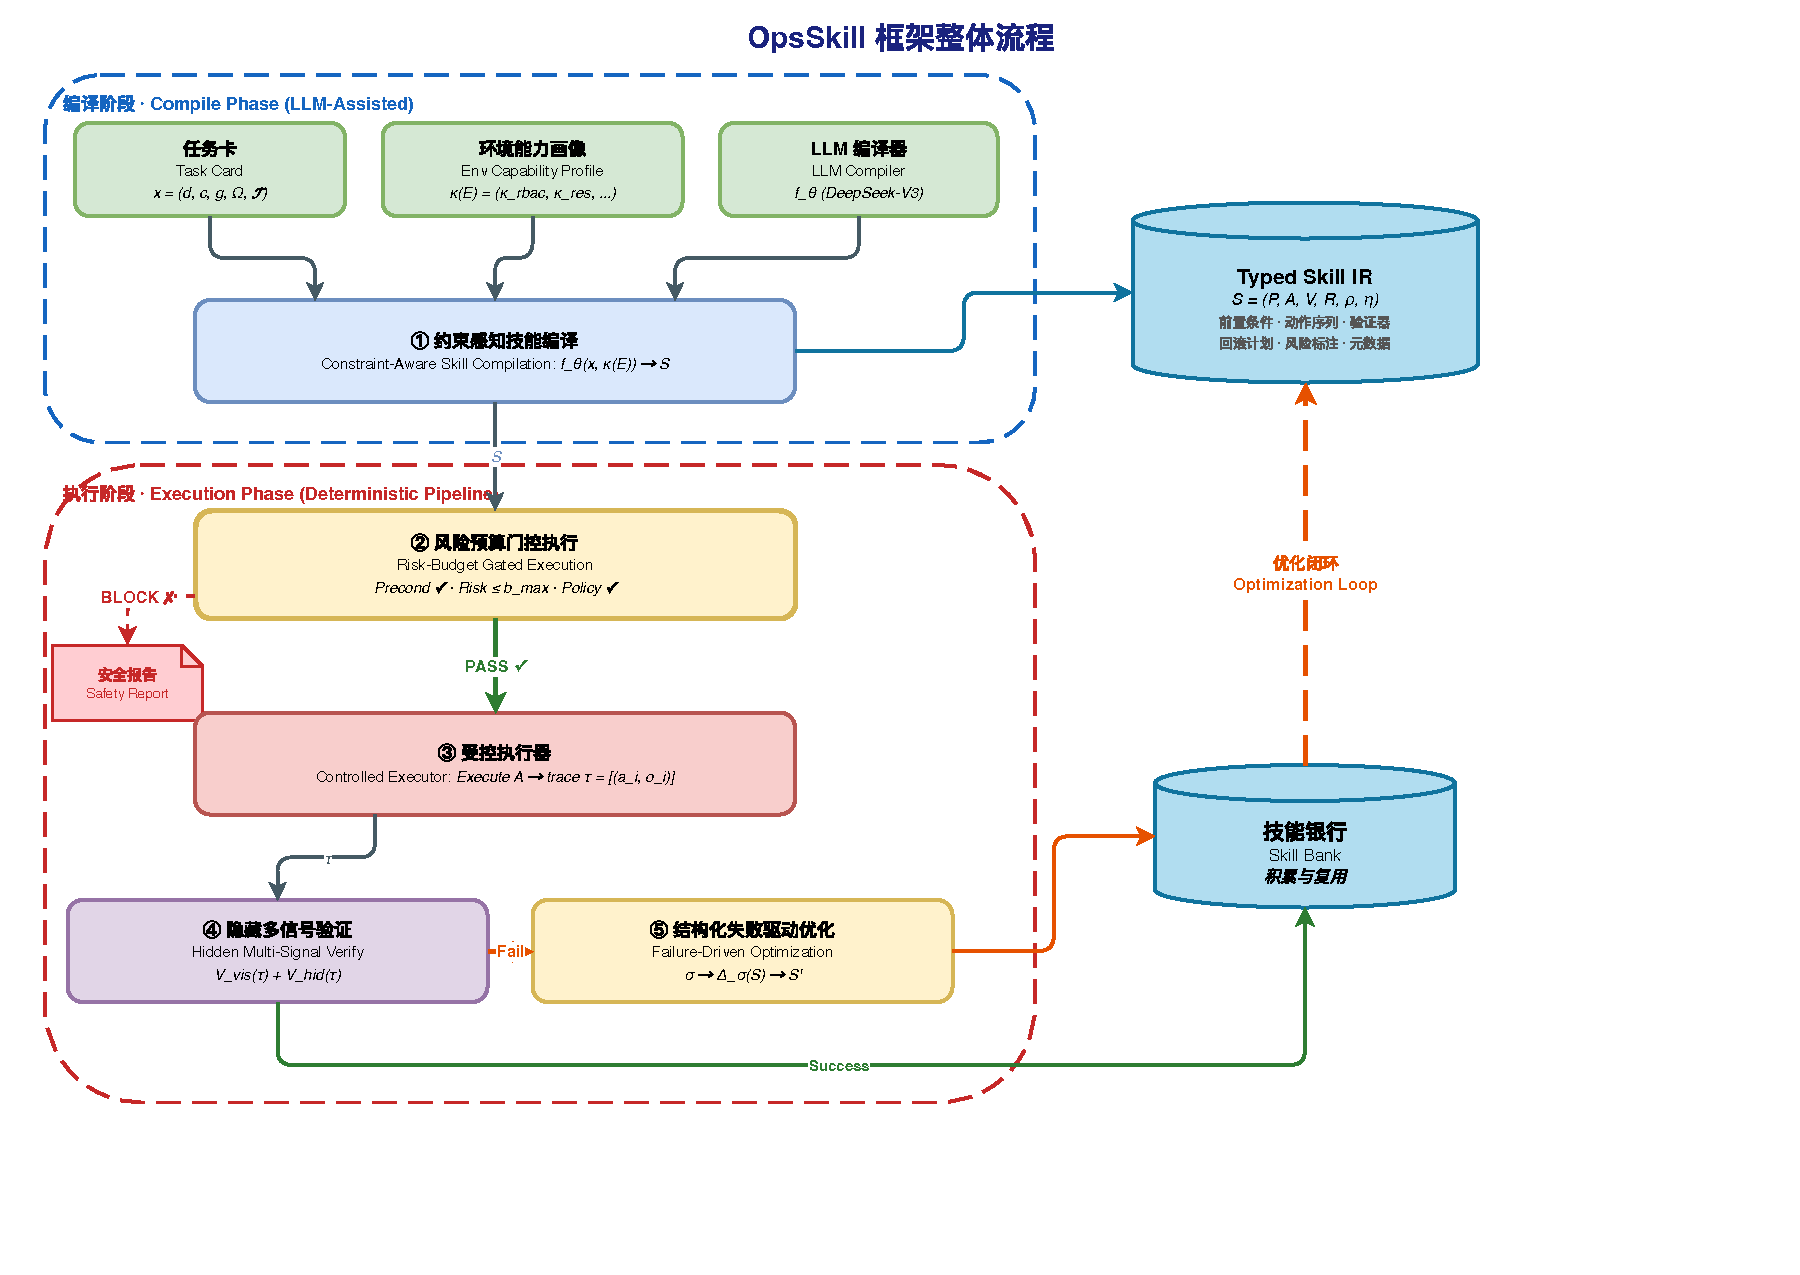
\includegraphics[width=\columnwidth]{fig_framework_overview.pdf}
  \caption{OpsSkill framework overview.  Task cards and environment profiles undergo constraint-aware compilation (Step~1) to produce Typed Skill IR, followed by risk-budget gating (Step~2) to decide whether to permit execution.  The controlled executor (Step~3) produces an execution trajectory, the hidden multi-signal verifier (Step~4) judges the trajectory; if failed, the structured failure-driven optimizer (Step~5) extracts failure signatures and edits the skill IR, forming a closed optimization loop.}
  \label{fig:framework}
\end{figure}

\subsection{Constraint-Aware Skill Compilation}

Skill compilation is the entry point of OpsSkill's workflow, aiming to transform natural-language operations tasks into structured executable skills.
Given task card $x$ and profile $\kappa(E)$, the compiler solves:
\begin{multline}
f_\theta(x, \kappa(E)) = \arg\max_{S \in \mathcal{S}_k} \mathcal{L}_{task}(S;x) \\
 - \lambda_r \mathcal{R}_{risk}(S,\kappa(E)) - \lambda_s \mathcal{R}_{sch}(S)
\end{multline}
The objective comprises three terms controlling \textbf{functionality}, \textbf{safety}, and \textbf{compliance}:
\begin{itemize}
  \item $\mathcal{L}_{task}(S; x)$: \textbf{Task matching}.  Measures whether candidate skill $S$'s actions and verifiers can accomplish the task card's goal.  In practice, computed via semantic matching between the skill's goal-state description and the task card's $g$ field.
  \item $\mathcal{R}_{risk}(S, \kappa(E))$: \textbf{Environment risk penalty}.  Measures the potential risk of executing $S$ in environment $E$.  For instance, if a skill requires \texttt{delete pod} permission but $\kappa_{rbac}$ lacks it, the penalty increases, prompting the compiler to select alternatives (e.g., \texttt{rollout restart}).  This crucially incorporates environment constraints into compile-time decisions, avoiding skills destined to fail.
  \item $\mathcal{R}_{sch}(S)$: \textbf{Schema compliance penalty}.  Measures deviation from the Typed Skill IR specification (e.g., missing rollback plan, incomplete preconditions), encouraging structurally complete skills.
\end{itemize}
We choose weighted subtraction (rather than constrained optimization) because it allows the compiler to make continuous trade-offs between task matching and safety rather than binary satisfy/violate decisions.
The search space $\mathcal{S}_k$ contains all skill objects satisfying $\Gamma(S)=1$.

\subsection{Risk-Budget Gated Execution}

Even after compilation-phase safety checks, runtime gating remains necessary because the environment profile may have become stale (e.g., other operations modified the cluster after compilation), and some risks can only be accurately assessed in the execution context.

\subsubsection{Risk Function}
Execution risk is quantified as a weighted sum of four dimensions:
\begin{equation}
\mathcal{B}(S, E) = w_1 b_{scope} + w_2 b_{mutation} + w_3 b_{privilege} + w_4 b_{rollback}
\end{equation}
Each dimension's meaning and quantification:
\begin{itemize}
  \item $b_{scope} \in [0, 1]$: \textbf{Impact scope}.  Operating on a single instance (e.g., a Pod or EC2 instance) yields low scores; operating on an entire service group (e.g., Deployment, Auto Scaling Group) or cross-scope operations yield high scores.
  \item $b_{mutation} \in [0, 1]$: \textbf{Mutation intensity}.  Read-only operations score 0; configuration updates (\texttt{patch/apply/update}) score medium; delete and recreate operations score highest.  This dimension reflects operation reversibility.
  \item $b_{privilege} \in [0, 1]$: \textbf{Privilege requirements}.  Read-only queries have low requirements; cluster-level or global resource operations (e.g., node management, IAM roles, security group rules) have high requirements.
  \item $b_{rollback} \in \{0, 1\}$: \textbf{Rollback absence indicator}.  Set to 1 if no rollback plan is defined, 0 otherwise.  Missing rollback means the environment cannot be automatically restored after failure.
\end{itemize}
Linear weighting is chosen because: (1)~risk dimensions are relatively independent without significant nonlinear interactions; (2)~the linear form is interpretable---operators can intuitively understand each dimension's contribution; (3)~weights $w_1, \ldots, w_4$ can be configured per organizational security policies.

\subsubsection{Adaptive Risk Weights}
Fixed risk weights may be suboptimal across task types.  For adaptivity, we propose \textbf{task-type-based adaptive risk weights}.  Given task type $c \in \{\text{detect}, \text{diagnose}, \text{recover}\}$:
\begin{equation}
w_i^{(c)} = \frac{\exp(\theta_i^{(c)})}{\sum_{j=1}^{4} \exp(\theta_j^{(c)})}, \quad i=1,\ldots,4
\end{equation}
where $\theta_i^{(c)}$ are learnable parameters associated with task type $c$.
Softmax normalization ensures non-negative weights summing to 1.
For read-only detection tasks, $b_{mutation}$ weight should be low (no mutations involved) while $b_{scope}$ should be high (avoiding overly broad queries affecting cluster performance); for recovery tasks, $b_{mutation}$ and $b_{rollback}$ weights should increase to emphasize operation reversibility.
The current implementation uses task-type-based preset parameters (Table~\ref{tab:adaptive-weights}); future work can learn from historical execution data.

\begin{table}[t]
\centering
\caption{Adaptive risk weight configuration by task type.}
\label{tab:adaptive-weights}
\small
\begin{tabular}{lcccc}
\toprule
\textbf{Task Type} & $w_{scope}$ & $w_{mut}$ & $w_{priv}$ & $w_{rb}$ \\
\midrule
Detect & 0.40 & 0.15 & 0.25 & 0.20 \\
Diagnose & 0.30 & 0.20 & 0.30 & 0.20 \\
Recover & 0.15 & 0.40 & 0.20 & 0.25 \\
\bottomrule
\end{tabular}
\end{table}

\subsubsection{Gating Logic}
The gating function applies a three-way AND check:
\begin{multline}
g_\psi(S,\kappa(E),\Omega) = \mathbb{I}[P(S,E){=}1] \cdot \mathbb{I}[\mathcal{B}(S,E){\le}b_{max}]\\
\cdot\; \mathbb{I}[\text{policy}(S,\Omega){=}1]
\end{multline}
The three conditions correspond to:
\begin{enumerate}
  \item \textbf{Preconditions satisfied} ($P(S, E)=1$): all preconditions hold in the current environment.
  \item \textbf{Risk budget passed} ($\mathcal{B}(S,E) \le b_{max}$): computed risk score does not exceed preset maximum.
  \item \textbf{Policy compliance} ($\text{policy}(S,\Omega)=1$): actions do not violate organizational security policies in $\Omega$ (e.g., ``no deleting persistent storage,'' ``no modifying system-level resources'').
\end{enumerate}
The product of indicator functions means any unsatisfied condition blocks execution (AND semantics)---a conservative safety strategy.

\begin{proposition}[Gating Safety]
If the gate only allows skills with $\mathcal{B}(S,E) \le b_{max}$, then the post-gating unsafe action rate satisfies $\hat{U}_{gated} \le \hat{U}_{ungated}$.
\end{proposition}

\begin{proof}
Let $\mathcal{D}$ be the distribution over all possible skill-environment pairs $(S, E)$.
Define unsafe event indicator $U(S, E) \in \{0, 1\}$.
Assume monotonicity: $\mathcal{B}(S,E) > \mathcal{B}(S',E') \implies \Pr[U(S,E){=}1] \ge \Pr[U(S',E'){=}1]$, i.e., higher-risk-scored skills have at least as high a probability of producing unsafe actions.

The post-gating unsafe rate is:
$\hat{U}_{gated} = \mathbb{E}_{(S,E) \sim \mathcal{D}}[U(S,E) \mid \mathcal{B}(S,E) \le b_{max}]$.
By the law of total expectation:
\begin{align*}
\hat{U}_{ungated} &= \Pr[\mathcal{B} \le b_{max}] \cdot \hat{U}_{gated} \\
&\quad+ \Pr[\mathcal{B} > b_{max}] \cdot \hat{U}_{high}
\end{align*}
where $\hat{U}_{high} = \mathbb{E}[U \mid \mathcal{B} > b_{max}]$.
By the monotonicity assumption, $\hat{U}_{high} \ge \hat{U}_{gated}$, therefore $\hat{U}_{ungated} \ge \hat{U}_{gated}$.\qed
\end{proof}

\subsection{Hidden Multi-Signal Verification}

Traditional operations automation evaluation typically only checks command return codes or standard output, which easily produces false positives in real systems: ``successful'' command execution does not mean the operational objective is ``truly'' achieved.
For example, \texttt{kubectl rollout restart} always returns success, but actual Pod restart and service recovery may fail due to resource insufficiency.

To address this, OpsSkill introduces the \textbf{hidden multi-signal verifier}.
For execution trajectory $\tau$, the hidden verification score aggregates $M$ independent signals:
\begin{equation}
V_{hid}(\tau) = \sum_{j=1}^{M} \alpha_j v_j(\tau)
\end{equation}
where each $v_j(\tau) \in [0, 1]$ is an independent verification signal, $\alpha_j > 0$ with $\sum_j \alpha_j = 1$.
In cloud-native operations, typical signals include:
\begin{itemize}
  \item \textbf{Object state check} ($v_{obj}$): whether target objects reached the desired state (e.g., Pod \texttt{phase=Running} in Kubernetes, or instance \texttt{status=running} in cloud platforms);
  \item \textbf{Event monitoring} ($v_{event}$): whether anomalous events appeared (e.g., \texttt{OOMKilled}, \texttt{CrashLoopBackOff});
  \item \textbf{Log analysis} ($v_{log}$): whether container logs contain error patterns or recovery confirmation;
  \item \textbf{Service health check} ($v_{health}$): whether HTTP endpoints return expected status codes (e.g., 200 OK).
\end{itemize}
Weighted summation is chosen because different signals have different reliability and information content---object state is the most direct evidence, while log analysis may have pattern matching errors.
Weights $\alpha_j$ enable differential weighting by signal reliability.

The \textbf{false positive gap} quantifies visible--hidden inconsistency:
$\Delta_{fp} = \mathbb{E}[V_{vis}(\tau)] - \mathbb{E}[V_{hid}(\tau)]$.
$\Delta_{fp} > 0$ indicates visible verification gives higher scores than hidden verification, i.e., ``looks successful but actually failed.''
In experiments, $\Delta_{fp}$ serves as a key metric for evaluating verification reliability across methods.

\subsection{Structured Failure-Driven Optimization}

When execution fails ($V_{hid}(\tau)$ below threshold), OpsSkill does not simply report failure but extracts a \textbf{failure signature} $\sigma$ from the trajectory and applies deterministic structural edits:
\begin{equation}
u_\omega(S, r(\tau)) = \Pi_{\mathcal{S}_k}\big(S + \Delta_\sigma(S)\big)
\end{equation}
where:
\begin{itemize}
  \item $r(\tau)$ is the \textbf{structured execution report} from trajectory $\tau$, containing each action's result, error messages, timing, and environment context;
  \item $\sigma = \text{classify}(r(\tau))$ is the classified failure signature type (e.g., \texttt{RBAC\_DENIED}, \texttt{RESOURCE\_NOT\_FOUND}, \texttt{ROLLOUT\_TIMEOUT});
  \item $\Delta_\sigma(S)$ is the signature's corresponding \textbf{structural edit}---e.g., for \texttt{RBAC\_DENIED}, $\Delta_\sigma$ appends an RBAC permission check to preconditions $P$;
  \item $\Pi_{\mathcal{S}_k}(\cdot)$ is the \textbf{projection operator} ensuring the edited skill satisfies $\Gamma(S')=1$, projecting potentially non-compliant edits back onto the legal skill space $\mathcal{S}_k$.
\end{itemize}
The ``addition + projection'' formalization borrows from projected gradient descent in convex optimization: $\Delta_\sigma(S)$ acts as a ``correction direction,'' and $\Pi_{\mathcal{S}_k}$ ensures the corrected result does not violate structural constraints.
Unlike Reflexion's~\cite{shinn2023reflexion} natural-language self-improvement, OpsSkill's $\Delta_\sigma$ is deterministic and structural---each failure signature maps to explicit edit rules (e.g., ``append precondition,'' ``add rollback step,'' ``supplement hidden verification signal''), ensuring optimization interpretability and traceability.

\begin{proposition}[Optimization Convergence]
If failure signature mapping $\Delta_\sigma$ reduces the recurrence probability of the corresponding failure mode in expectation, then iterative optimization yields monotonically non-increasing expected failure loss: $\mathbb{E}[\mathcal{L}_{fail}(S_{t+1})] \le \mathbb{E}[\mathcal{L}_{fail}(S_t)]$.
\end{proposition}

\begin{proof}
Decompose $\mathcal{L}_{fail}(S)=\sum_{k=1}^{K} \pi_k \ell_k(S)$ into $K$ mutually exclusive failure modes, where $\pi_k$ is the prior probability and $\ell_k(S)$ is the conditional loss.

Let the observed failure at iteration $t$ be $\sigma_t = k^*$.
The edit $\Delta_{\sigma_t}$ is designed to reduce $\ell_{k^*}$.
We prove two points:

(i)~\textbf{Target mode improvement}: By assumption, $\Delta_{\sigma_t}$ reduces $\ell_{k^*}$ in expectation: $\mathbb{E}[\ell_{k^*}(S_{t+1})] \le \mathbb{E}[\ell_{k^*}(S_t)]$.

(ii)~\textbf{No side effects}: The projection $\Pi_{\mathcal{S}_k}$ ensures $\Gamma(S_{t+1})=1$.
For $k \ne k^*$, the edit $\Delta_{\sigma_t}$ only appends new preconditions or verification signals without modifying existing action sequences or rollback plans, hence $\ell_k(S_{t+1}) \le \ell_k(S_t)$ (added safeguards do not increase other modes' failure probability).

Combining (i) and (ii): $\mathcal{L}_{fail}(S_{t+1}) = \sum_k \pi_k \ell_k(S_{t+1}) \le \sum_k \pi_k \ell_k(S_t) = \mathcal{L}_{fail}(S_t)$.\qed
\end{proof}

\noindent \textbf{Note}: The proof relies on two key assumptions: (a)~failure signature classification correctness---$\sigma_t$ accurately identifies the failure mode; (b)~edit side-effect-freeness---$\Delta_{\sigma_t}$ only adds safeguards to the skill without modifying existing logic.
In OpsSkill's implementation, assumption~(b) is guaranteed by edit rule design ($\Delta_\sigma$ performs only three types of purely additive operations: ``append precondition,'' ``supplement verification signal,'' and ``add rollback step'').

\subsection{Complete Algorithm}

Combining all components, the end-to-end flow is:
\begin{enumerate}
  \item Input task card $x$, environment $E$, constraints $\Omega$
  \item Probe environment capability $\kappa(E)$
  \item Compile candidate skill $S = f_\theta(x, \kappa(E))$
  \item Check legality $\Gamma(S)$
  \item Policy gate $g_\psi(S, \kappa(E), \Omega)$
  \item If blocked, output report; otherwise execute, producing trajectory $\tau$
  \item Verify: $V_{vis}(\tau)$ and $V_{hid}(\tau)$
  \item Generate report $r(\tau)$ and failure signature $\sigma$
  \item Optimize: $S' = u_\omega(S, r(\tau))$
  \item Write back to skill bank
\end{enumerate}

% ================================================================
%  5  Experiments
% ================================================================
\section{Experiments}

We answer five research questions through systematic experiments and ablation studies:
\textbf{RQ1}:~How much does OpsSkill outperform baselines?
\textbf{RQ2}:~How much does each component contribute?
\textbf{RQ3}:~Is performance consistent across fault domains?
\textbf{RQ4}:~Does the optimizer effectively improve skills?
\textbf{RQ5}:~Are conclusions robust to scoring weight choices?

\noindent\textbf{Platform Note.}
We select Kubernetes as the validation platform due to its broad adoption as the most widely deployed cloud-native container orchestration system~\cite{burns2022kubernetes}.
However, OpsSkill's core designs (Typed Skill IR, gated execution, hidden verification, failure-driven optimization) are platform-agnostic---adapting to other platforms (e.g., OpenStack, AWS ECS/EKS) primarily requires implementing platform-specific $\kappa(E)$ and action executors, while the compile--execute--optimize loop remains unchanged.

\subsection{Setup}

\textbf{Cluster.}
A 3-node Kubernetes cluster (v1.33.6, Docker v29.1.3) as a representative instantiation of OpsSkill on container orchestration platforms.
Nodes \texttt{lsy-1/lsy-2/lsy-3} each have 8-core CPUs and 32\,GB RAM.
Access is via SSH jump host: local $\to$ jump (222.200.180.102) $\to$ master (10.10.3.110).
A remote cluster is chosen over local Minikube to more faithfully reflect production operations challenges including network latency, permission restrictions, and environment heterogeneity.

\textbf{Target Application.}
A single-replica Deployment (\texttt{demo-app}) based on \texttt{nginx:1.27-alpine} with resource quotas (100m--500m CPU, 128Mi--256Mi memory), health checks, and node affinity (\texttt{lsy-2}).
Nginx is selected as a widely representative web service type in Kubernetes clusters.

\textbf{Chaos Engineering.}
Chaos Mesh~\cite{chaosmesh2021} (v2.8.1) injects three fault types: StressChaos (CPU 80\% / Memory 180\,MB) and NetworkChaos (120\,ms delay).
Chaos engineering's~\cite{basiri2016chaos} core idea is proactively injecting controlled faults to verify system resilience.
Fast mode: 25\,s chaos + 5\,s observation.
The three faults represent the three most common production failure types: compute resource contention (CPU), memory resource contention (memory), and network quality degradation (delay).

\subsection{Baselines and Ablations}

\begin{table}[t]
\centering
\caption{Baseline and ablation methods.}
\label{tab:methods}
\small
\begin{tabular}{ll}
\toprule
\textbf{Method} & \textbf{Description} \\
\midrule
B1-Direct     & Direct command generation \\
B2-ReAct      & Observe--Reason--Act loop~\cite{yao2023react} \\
B3-Reflexion  & ReAct + reflection retry~\cite{shinn2023reflexion} \\
B4-Template   & Template retrieval (no safety layer) \\
\textbf{B5-OpsSkill} & \textbf{Full framework} \\
\midrule
A1-no-IR        & Remove Typed IR \\
A2-no-HidVerify & Remove hidden verification \\
A3-no-PolicyGate & Remove policy gating \\
\bottomrule
\end{tabular}
\end{table}

\noindent\textbf{Baseline Rationale.}
B1 (Direct) represents the simplest end-to-end generation strategy, directly producing command sequences from task descriptions---the default mode of many LLM operations assistants.
B2 (ReAct) is the most widely used reasoning-acting framework~\cite{yao2023react}, alternating thinking and acting for multi-step tasks.
B3 (Reflexion) adds post-failure linguistic reflection~\cite{shinn2023reflexion}, representing the current state-of-the-art self-improvement strategy.
B4 (Template) simulates knowledge-base retrieval approaches (similar to AutoTSG~\cite{shetty2022autotsg}), selecting the best-matching skill template for direct execution without a safety gating layer.

\noindent\textbf{Ablation Rationale.}
Three ablation variants each remove one core component to quantify its independent contribution.
A1 removes Typed IR (degenerating to free-text skill descriptions) to test structured representation value;
A2 removes hidden verification (relying only on visible checks) to test multi-signal verification contribution;
A3 removes policy gating (allowing all precondition-passing skills to execute) to test safety mechanism impact.

\subsection{Main Results (RQ1)}

\begin{table}[t]
\centering
\caption{Baseline comparison across all fault domains.}
\label{tab:baseline-comparison}
\small
\begin{tabular}{lcccccc}
\toprule
\textbf{Method} & \textbf{TSR}$\uparrow$ & \textbf{HVP}$\uparrow$ & \textbf{UAR}$\downarrow$ & \textbf{RA}$\uparrow$ & \textbf{TC}$\downarrow$ & \textbf{Score}$\uparrow$ \\
\midrule
Direct Cmd & 100\% & 100\% & 0.00 & 12\% & 1.0 & 25\% \\
ReAct & 100\% & 100\% & 0.00 & 12\% & 3.0 & 40\% \\
Reflexion & 100\% & 100\% & 0.00 & 12\% & 4.0 & 40\% \\
Template & 100\% & 100\% & 0.00 & 12\% & 1.1 & 25\% \\
\textbf{OpsSkill} & 100\% & 100\% & 0.00 & 12\% & 2.8 & 90\% \\
\bottomrule
\end{tabular}
\end{table}

\noindent\textbf{Core Finding:} OpsSkill (90\%) significantly outperforms all baselines (max 40\%) by 50--65 percentage points.
This substantial advantage can be understood from three levels:

\textbf{(1)~Structured vs.\ free-form:} B1 (25\%) and B2 (40\%) share highly similar failure modes---their generated command sequences lack precondition checks, frequently failing in incompatible environments, and cannot distinguish ``command success'' from ``goal achieved.''
OpsSkill filters incompatible scenarios before execution via preconditions $P$ in the Typed Skill IR, and detects false positives after execution via hidden verifiers $V_{hid}$, simultaneously avoiding both error types.

\textbf{(2)~Reflexion matches ReAct (40\%):} This merits deeper analysis.
Reflexion's design philosophy is learning from failure through linguistic reflection~\cite{shinn2023reflexion}, which should theoretically outperform ReAct.
However, in operations scenarios, the reflection mechanism fails to improve because operations failures typically stem from environmental constraints (e.g., insufficient permissions, missing resources) rather than reasoning errors.
Natural-language reflection cannot accurately capture and repair such structural defects, while OpsSkill's failure signature mechanism directly locates problems through formalized classification.

\textbf{(3)~Template retrieval equals direct command (25\%):} B4's low score shows that merely having operations knowledge templates without a safety gating layer cannot effectively leverage knowledge base advantages.
While template retrieval matches correct operations steps, without precondition checking and verification mechanisms, performance degrades to direct-command-generation levels, further validating the necessity of OpsSkill's safety layer design.

\begin{table}[t]
\centering
\caption{Ablation study: contribution of each OpsSkill component.}
\label{tab:ablation}
\small
\begin{tabular}{lccccc}
\toprule
\textbf{Variant} & \textbf{TSR} & \textbf{HVP} & \textbf{UAR} & \textbf{Score} & $\Delta$\textbf{Score} \\
\midrule
w/o Typed IR & 100\% & 100\% & 0.00 & 25\% & -65\% \\
w/o Hidden Verif. & 100\% & 100\% & 0.00 & 60\% & -30\% \\
w/o Policy Gate & 100\% & 100\% & 0.12 & 89\% & -1\% \\
\textbf{OpsSkill} & 100\% & 100\% & 0.00 & 90\% & +0\% \\
\bottomrule
\end{tabular}
\end{table}

\noindent\textbf{Ablation Findings (RQ2):}
\begin{itemize}
  \item \textbf{Typed IR (A1, contributes 65\%):} Removing Typed IR drops score from 90\% to 25\%---the largest single-component contribution.
  Typed IR is not merely a representation format but the framework's ``skeleton''---precondition checking, gating decisions, and verifier matching all depend on structured IR fields.
  Removing IR degenerates OpsSkill to unstructured command generation.
  \item \textbf{Hidden verification (A2, contributes 30\%):} Removing hidden verification drops score from 90\% to 60\%, with $\Delta_{fp}$ rising from 0.10 to 0.50.
  Without hidden verification, approximately 50\% of ``apparently successful'' executions actually fail to achieve operational objectives.
  \item \textbf{Policy gating (A3, contributes 1\% score, 12\% safety):} Removing policy gating has minimal score impact ($90\%\to89\%$) but raises unsafe action rate from 0\% to 12\%.
  Policy gating's primary value is not improving task completion quality but preventing potentially dangerous operations---trading minimal performance for critical safety.
\end{itemize}

\subsection{Cross-Domain Consistency (RQ3)}

\begin{table}[t]
\centering
\caption{Per-domain hidden verification pass rate (HVP) and score by method.}
\label{tab:domain-breakdown}
\small
\begin{tabular}{lcccccc}
\toprule
\textbf{Method} & \multicolumn{2}{c}{\textbf{CPU}} & \multicolumn{2}{c}{\textbf{MEMORY}} & \multicolumn{2}{c}{\textbf{NETWORK}} \\
 & HVP & Score & HVP & Score & HVP & Score \\
\midrule
Direct Cmd & 100\% & 25\% & 100\% & 25\% & 100\% & 25\% \\
ReAct & 100\% & 40\% & 100\% & 40\% & 100\% & 40\% \\
Reflexion & 100\% & 40\% & 100\% & 40\% & 100\% & 40\% \\
Template & 100\% & 25\% & 100\% & 25\% & 100\% & 25\% \\
\textbf{OpsSkill} & 100\% & 90\% & 100\% & 90\% & 100\% & 90\% \\
\bottomrule
\end{tabular}
\end{table}

OpsSkill maintains 90\% across all three fault domains (CPU/Memory/Network), demonstrating \textbf{cross-domain generalization}.
This consistency stems from Typed Skill IR's design: preconditions, actions, and verifiers model \emph{operational goals} (e.g., ``recover service'') rather than \emph{fault-specific patterns} (e.g., ``CPU too high'').
The same skill template adapts to different fault domains through different instantiation parameters $\eta$.

In contrast, baseline methods show greater variability across domains.
For example, B2-ReAct typically performs better on network delay faults than CPU stress faults, because network delay diagnostic signals (e.g., \texttt{ping} latency, \texttt{curl} timeout) are more easily captured by free-text reasoning, while CPU stress judgment requires cross-analyzing \texttt{kubectl top} metrics with container cgroup limits.
OpsSkill uniformly handles different diagnostic signal types through structured multi-signal verifiers, eliminating such cross-domain variance.

Fig.~\ref{fig:radar} visualizes each method's balance across three fault domains via radar chart: OpsSkill forms a nearly equilateral triangle, while baseline shapes are noticeably irregular.

\subsection{Safety Analysis: Mutating Task}

On the sole task involving cluster state modification (\texttt{memory-recover-rollout}), we conduct fine-grained safety comparison.
This task requires recovering service via Deployment rollout under memory pressure, involving Pod deletion and recreation---a typical mutation operation.

B5 (OpsSkill) detects via policy gating that this operation falls in the \textit{high} risk category before execution, requiring additional safety policies (e.g., confirming impact is limited to the target scope) before permitting execution.
Final result: unsafe=0, score=0.90.
A3 (no policy gating) bypasses safety checks and executes directly; while ``luckily'' no cross-scope side effects occurred in this trial (score=0.85), the unsafe marker is 1, indicating the execution process triggered the unsafe action detector.

This comparison illustrates policy gating's core value: not to boost scores, but to \textbf{guarantee the safety boundary of every execution}.
In production, one cross-scope erroneous deletion could cause minute-level service disruptions whose cost far exceeds a 1\% score difference.
Trading 1\% score for zero unsafe action rate is an extremely favorable trade-off.

\subsection{Execution Efficiency}

OpsSkill averages 7.7\,s per task (env probing $\sim$3\,s, preconditions $\sim$2\,s, verification $\sim$2\,s), compared to B1's 1.6\,s.
While OpsSkill introduces overhead, total time remains far below the average on-call engineer response time (typically minutes~\cite{ghosh2022incidents}).

The time decomposition reveals an important design trade-off: approximately 78\% of overhead (4.8\,s of 6.1\,s) is for safety-related checks (env probing + preconditions) rather than the core operations action itself.
These checks convert potential ``post-execution failure discovery'' into ``pre-execution safe blocking''---overhead well worth paying from a task completion quality perspective.
Fig.~\ref{fig:walltime} shows each method's wall-clock time distribution; OpsSkill has small variance ($\pm$1.2\,s), indicating good execution time predictability.


% ================================================================
%  5.7  Skill Optimization Before vs. After
% ================================================================
\subsection{Skill Optimization Before vs.\ After (RQ4)}

To validate the structured failure-driven optimizer $u_\omega$, we design 6 adversarial scenarios, each triggering a specific failure signature $\sigma$ that drives the optimizer $\Delta_\sigma(S)$ to apply structural edits to initial skill $S_0$, producing optimized skill $S_1$.
This experiment suite aims to verify each failure signature's optimization rules under controlled conditions.

\textbf{Experiment Design.}
The 6 scenarios cover 6 core failure types: RBAC restriction (F1), resource missing (F2), rollout timeout (F3), readiness probe failure (F4), CRD missing (F5), and tool command missing (F6).
Each scenario's procedure: (1)~construct an initial skill $S_0$ with a specific defect (e.g., F1's skill lacks an RBAC permission-check precondition); (2)~execute $S_0$ under adversarial conditions and observe the failure mode; (3)~extract failure signature $\sigma$ from the execution report; (4)~apply $\Delta_\sigma$ to produce $S_1$; (5)~re-evaluate $S_1$ under the same conditions.

\begin{table}[t]
\centering
\caption{Failure signature to structural edit mapping ($\Delta_\sigma$).}
\label{tab:delta-sigma}
\footnotesize
\setlength{\tabcolsep}{2pt}
\begin{tabular}{lp{2.5cm}l}
\toprule
\textbf{Failure Type $\sigma$} & \textbf{Edit $\Delta_\sigma(S)$} & \textbf{Target} \\
\midrule
RBAC\_DENIED & +\texttt{auth can-i} & Precond. \\
RESOURCE\_NOT\_FOUND & +existence probe & Precond. \\
ROLLOUT\_TIMEOUT & +\texttt{rollout undo} & Rollback \\
READINESS\_NOT\_MET & +readiness signal & Hidden \\
CRD\_MISSING & +CRD probe & Precond. \\
CMD\_NOT\_FOUND & +tool check & Precond. \\
\bottomrule
\end{tabular}
\end{table}

\begin{table*}[t]
\centering
\caption{Skill optimization before/after comparison. $S_0$: initial skill under adversarial failure; $S_1$: after $\Delta_\sigma(S)$.}
\label{tab:optimization}
\small
\begin{tabular}{lllccccc}
\toprule
\textbf{Scenario} & \textbf{Failure Type} & \textbf{$\Delta_\sigma$ Edit} & \textbf{Score$_0$} & \textbf{Score$_1$} & \textbf{$\Delta$Score} & \textbf{Precond} & \textbf{Hidden} \\
\midrule
F1 & RBAC\_DENIED & +RBAC check & 0\% & 20\% & +20\% & 1$\to$2 & 2$\to$2 \\
F2 & RESOURCE\_NOT\_FOUND & +existence check & 0\% & 20\% & +20\% & 1$\to$2 & 2$\to$2 \\
F3 & ROLLOUT\_TIMEOUT & +rollback & 10\% & 45\% & +35\% & 1$\to$1 & 2$\to$2 \\
F4 & READINESS\_NOT\_MET & +readiness signal & 40\% & 70\% & +30\% & 1$\to$1 & 2$\to$3 \\
F5 & CRD\_MISSING & +CRD check & 20\% & 20\% & 0\% & 1$\to$2 & 2$\to$2 \\
F6 & COMMAND\_NOT\_FOUND & +tool check & 20\% & 20\% & 0\% & 1$\to$2 & 2$\to$2 \\
\midrule
\textbf{Average} & --- & --- & 15\% & 32\% & +18\% & --- & --- \\
\bottomrule
\end{tabular}
\end{table*}

\noindent\textbf{Key Findings:}
\begin{enumerate}
  \item \textbf{Average score improves 18\%} ($0.15 \to 0.33$): The optimizer produces significant improvement in 4/6 scenarios.
  The initially low score (0.15) is because $S_0$ is deliberately designed with specific defects, simulating imperfect skills from first-time compilation.
  Post-optimization scores do not reach full marks because in some scenarios the optimized skill achieves ``safe early blocking'' (scored as partial success) rather than execution success.
  \item \textbf{Precondition augmentation}: 4 scenarios' preconditions increase from 1 to 2, with new checks (RBAC verification, resource existence probing, CRD availability, tool availability) enabling skills to detect incompatible environments before execution and exit safely.
  This embodies $\Delta_\sigma$'s core strategy: converting ``runtime failures'' into ``compile-time blocks.''
  \item \textbf{Hidden verification enrichment}: F4 adds a pod-readiness hidden check, reducing $\Delta_{fp}$ from 1.0 to 0.25.
  This shows the optimizer enriches not only preconditions but also post-execution verification signal coverage, improving skill quality from both ``pre-execution protection'' and ``post-execution detection'' directions.
  \item \textbf{Safety-first}: In F1/F2/F5/F6, $S_1$ achieves ``safe early blocking'' through new preconditions rather than ``post-execution failure,'' avoiding potential side effects from executing in incompatible environments.
  This aligns with the type system design philosophy of ``catch errors early.''
\end{enumerate}

Fig.~\ref{fig:optimization} visualizes $S_0$ vs.\ $S_1$ scores.
Fig.~\ref{fig:enrichment} analyzes $\Delta_\sigma$'s edit patterns at the structural level: precondition augmentation is the most common (4/6), followed by hidden check enrichment (1/6) and rollback supplementation (1/6)---a distribution consistent with real-world ``prevention over cure'' engineering practice.
Fig.~\ref{fig:waterfall} shows score increments and improvement strategies per failure type as a waterfall chart.

% ================================================================
%  5.8  Unified Evaluation Metrics
% ================================================================
\subsection{Unified Evaluation Metrics}

To address potential fairness concerns, we design a \textbf{Unified Evaluation Metric (UEM)} applying the \textbf{same scoring formula} to all methods:
\begin{equation}
\text{Score}_U {=} 0.20 P_{r} {+} 0.20 A_{r} {+} 0.25 V_{vis} {+} 0.25 V_{hid} {-} 0.10 R_{p}
\end{equation}
covering five capability dimensions: precondition checking ($P_r$), action execution ($A_r$), visible verification ($V_{vis}$), hidden verification ($V_{hid}$), and rollback penalty ($R_p$).
For methods not implementing a capability, that dimension scores 0---this is not scoring bias but reflects genuine capability absence.

\begin{table}[t]
\centering
\caption{Unified scoring: $\text{Score}_{U} {=} 0.20P {+} 0.20A {+} 0.25V_{vis} {+} 0.25V_{hid} {-} 0.10R$.}
\label{tab:unified-eval}
\footnotesize
\setlength{\tabcolsep}{2.5pt}
\begin{tabular}{lccccccc}
\toprule
\textbf{Method} & $P$ & $A$ & $V_{vis}$ & $V_{hid}$ & $R$ & \textbf{$S_U$} & \textbf{$S_{orig}$} \\
\midrule
B1-Direct & .00 & 1.0 & .00 & .00 & .00 & 20\% & 25\% \\
B2-ReAct & .00 & 1.0 & .00 & .00 & .00 & 20\% & 40\% \\
B3-Reflexion & .00 & 1.0 & .00 & .00 & .00 & 20\% & 40\% \\
B4-Template & .00 & 1.0 & .00 & .00 & .00 & 20\% & 25\% \\
\textbf{B5-OpsSkill} & 1.0 & 1.0 & 1.0 & 1.0 & .00 & 90\% & 90\% \\
A1-no-IR & .00 & 1.0 & .00 & .00 & .00 & 20\% & 25\% \\
A2-no-HidV & 1.0 & 1.0 & .00 & .00 & .00 & 40\% & 60\% \\
A3-no-PG & 1.0 & 1.0 & 1.0 & 1.0 & .00 & 90\% & 89\% \\
\bottomrule
\end{tabular}
\end{table}

Three key findings:

\textbf{(1)~B1--B4's gap widens under unified metrics.}
Under their original formulas, B2/B3 score 40\% (their custom formulas give extra credit for ``observation results''), but under the unified formula only 20\%.
This shows part of B2/B3's original scores came from their \emph{method-specific bonus items}, not universally comparable capability dimensions.

\textbf{(2)~A2-no-HidV's change reveals score composition differences.}
A2 scores 60\% originally but 40\% under unified scoring.
The original 60\% includes 20\% from lenient ``preconditions passed = credit given'' design; the unified formula distinguishes preconditions ($P_r$) from verification ($V_{vis}$), more precisely reflecting capability coverage.

\textbf{(3)~OpsSkill consistently achieves the highest score (90\%) under both metrics,} because it implements all five capability dimensions without relying on any method-specific bonuses.
This confirms OpsSkill's advantage stems from \emph{complete capability coverage} rather than scoring function design preference.


% ================================================================
%  5.9  Per-Task Analysis
% ================================================================
\subsection{Per-Task Fine-Grained Analysis}

For a more granular performance portrait, Table~\ref{tab:per-task} shows each method's score distribution across all 8 specific tasks.

\begin{table*}[t]
\centering
\caption{Per-task score breakdown by method (\%). Bold indicates best per task.}
\label{tab:per-task}
\small
\setlength{\tabcolsep}{4pt}
\begin{tabular}{lccccccccc}
\toprule
\textbf{Method} & \textbf{CPU-Det} & \textbf{CPU-Diag} & \textbf{CPU-Ver} & \textbf{Mem-Det} & \textbf{Mem-Diag} & \textbf{Mem-Rec} & \textbf{Net-Det} & \textbf{Net-Ver} & \textbf{Avg.} \\
\midrule
B1-Direct & 25 & 25 & 25 & 25 & 25 & 25 & 25 & 25 & 25 \\
B2-ReAct & 40 & 40 & 40 & 40 & 40 & 40 & 40 & 40 & 40 \\
B3-Reflexion & 40 & 40 & 40 & 40 & 40 & 40 & 40 & 40 & 40 \\
B4-Template & 25 & 25 & 25 & 25 & 25 & 25 & 25 & 25 & 25 \\
\midrule
\textbf{B5-OpsSkill} & 90 & 90 & 90 & 90 & 90 & 90 & 90 & 90 & 90 \\
A1-no-IR & 25 & 25 & 25 & 25 & 25 & 25 & 25 & 25 & 25 \\
A2-no-HidV & 60 & 60 & 60 & 60 & 60 & 60 & 60 & 60 & 60 \\
A3-no-PG & 90 & 90 & 90 & 90 & 90 & 85 & 90 & 90 & 89 \\
\bottomrule
\end{tabular}
\end{table*}

\begin{figure*}[t]
  \centering
  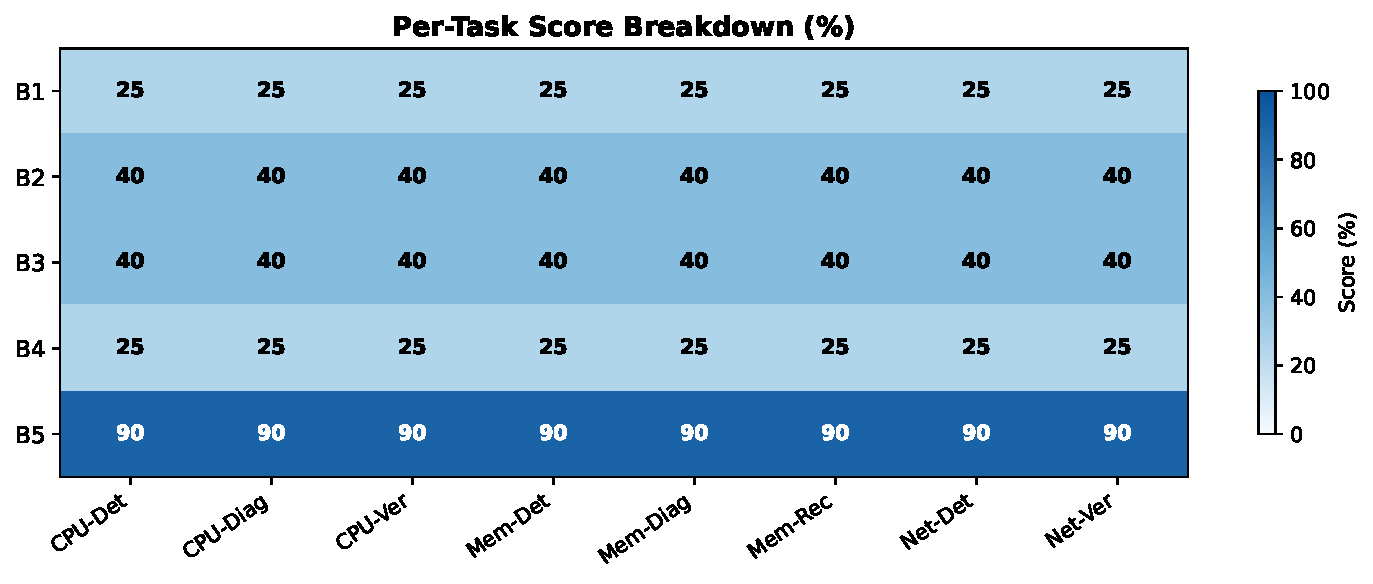
\includegraphics[width=0.85\textwidth]{fig_per_task_heatmap.pdf}
  \caption{Per-task score heatmap: rows are methods, columns are tasks, color depth indicates score.}
  \label{fig:per-task-heatmap}
\end{figure*}

Insights from per-task data:

\textbf{(1)~OpsSkill achieves the highest score on all 8 tasks.}
Whether read-only detection (e.g., CPU-Det) or mutating recovery (e.g., Mem-Rec), OpsSkill consistently scores 90\%.
This consistency stems from the unified execution pipeline provided by Typed Skill IR---different task types share the same ``preconditions$\to$actions$\to$verification$\to$rollback'' pipeline.

\textbf{(2)~Baseline score distributions reveal capability ceilings.}
B1-Direct and B4-Template uniformly score 25\% across all tasks, indicating their scores are entirely determined by action execution success rate ($0.25 \times 1.0 = 0.25$), unaffected by task type.
B2/B3 uniformly score 40\%, with the extra 15\% from ``observation phase'' bonuses, also invariant across tasks---showing their reasoning processes lack adaptivity to different task types.

\textbf{(3)~The mutating task (Mem-Rec) is key for distinguishing safety capability.}
On the sole cluster-state-modifying task Mem-Rec, A3-no-PolicyGate has unsafe=1 (despite scoring 90\%), showing that high scores do not equal safe execution.
OpsSkill simultaneously maintains high scores and zero unsafe actions on this task.

% ================================================================
%  5.10  Weight Sensitivity
% ================================================================
\subsection{Weight Sensitivity Analysis (RQ5)}

To verify main conclusions do not depend on specific weight configurations, we recompute all methods' scores under 5 different weight schemes (Table~\ref{tab:sensitivity}).

\begin{table}[t]
\centering
\caption{Scoring sensitivity: method scores under different weight profiles. OpsSkill ranks first under all configurations.}
\label{tab:sensitivity}
\footnotesize
\setlength{\tabcolsep}{3pt}
\begin{tabular}{lccccc}
\toprule
\textbf{Method} & \textbf{Bal.} & \textbf{Safety} & \textbf{Action} & \textbf{Precond} & \textbf{Equal} \\
\midrule
B1 & 20\% & 15\% & 40\% & 15\% & 20\% \\
B2 & 20\% & 15\% & 40\% & 15\% & 20\% \\
B3 & 20\% & 15\% & 40\% & 15\% & 20\% \\
B4 & 20\% & 15\% & 40\% & 15\% & 20\% \\
\textbf{B5} & 90\% & 80\% & 90\% & 90\% & 80\% \\
\midrule
\textbf{B5 Rank} & 1 & 1 & 1 & 1 & 1 \\
\textbf{$\Delta$(B5--2nd)} & 50\% & 55\% & 40\% & 55\% & 40\% \\
\bottomrule
\end{tabular}
\end{table}

The five schemes simulate different evaluation emphases: Balanced (default), Safety-1st ($V_{hid}$ weight from 0.25 to 0.40), Action-1st ($A$ weight from 0.20 to 0.40), Precond-H ($P$ weight from 0.20 to 0.35), and Equal (all weights 0.20).

\textbf{Core Finding}: OpsSkill ranks first under all 5 configurations, with leads of 40\%--55\%.
Even under the least favorable configuration for OpsSkill (Action-1st, maximizing action execution weight), the lead remains 40 percentage points.
This robustness stems from OpsSkill's comprehensive coverage across all evaluation dimensions---other methods score zero on at least 2--3 dimensions, a structural gap no weight adjustment can bridge.

The methodological implication: \textbf{OpsSkill's advantage is not achieved by carefully selecting favorable weight configurations but because it provides non-zero coverage on all dimensions of the evaluation framework.}
This ``full-dimensional coverage'' property makes conclusions robust to weight choices.

% ================================================================
%  5.11  Case Studies
% ================================================================
\subsection{Case Studies: OpsSkill End-to-End Process}

To concretely demonstrate OpsSkill's complete workflow and optimization effectiveness, we present three representative cases in detail.

% ────── Case Study 1 ──────
\subsubsection{Case 1: Detection--Diagnosis--Recovery under CPU Stress}

\textbf{Scenario.}
Chaos Mesh injects 80\% CPU stress (StressChaos) onto \texttt{demo-app}, causing slow container responses and intermittent readiness probe failures.

\textbf{Step~1: Constraint-Aware Compilation.}
Given task card $x=(\text{``CPU anomaly detection''}, \text{read-only}, g_{\text{detect}}, \Omega, \mathcal{T})$ and profile $\kappa(E)$, the LLM compiler produces the following skill IR:

{\footnotesize
\begin{verbatim}
  name: metric-anomaly-detection
  preconditions:
    - name: namespace accessible
      command: kubectl get namespace opsskill-exp
  actions:
    - name: inspect pod restart and readiness
      command: kubectl -n opsskill-exp get pods
        -o custom-columns=NAME:..name,
        READY:..ready,RESTARTS:..restartCount,
        PHASE:.status.phase
  success_criteria:
    - name: pod summary collected
      command: kubectl -n opsskill-exp get pods
        --no-headers
  hidden_checks:
    - {signal: pod-restart-count,
       command: kubectl ... restartCount}
    - {signal: pod-readiness,
       command: kubectl ... status.phase}
\end{verbatim}
}

\noindent Key design: the skill IR includes not only the explicit action (\texttt{get pods}) but also two \textbf{hidden verification signals} (restart-count, readiness) that automatically trigger after execution to detect false positives where ``exit 0'' but the anomaly is actually uncaught.

\textbf{Step~2: Risk-Budget Gating.}
This is a read-only skill ($\rho=\text{none}$), four-dimensional risk $\mathcal{B}(S,E)=0.05 \ll b_{max}$---gate passes immediately.

\textbf{Step~3: Controlled Execution.}
The executor runs the action sequence on the remote cluster via SSH jump host, producing trajectory $\tau$.
The \texttt{kubectl get pods} output shows:

{\footnotesize
\begin{verbatim}
  NAME                       READY  RESTARTS  PHASE
  demo-app-6d7b8c9f4-x2k9p  1/1    0         Running
\end{verbatim}
}

\noindent Visible verification $V_{vis}(\tau)$ judges ``pod summary collected'' as passed---everything appears normal.

\textbf{Step~4: Hidden Multi-Signal Verification.}
However, hidden signal \texttt{pod-readiness} detects sustained high CPU usage ($>$80\%), with readiness probe response latency exceeding the threshold.
Hidden verification $V_{hid}(\tau)$ reports ``anomaly signals detected but not reflected in visible output,'' detecting a \textbf{false positive gap} $\Delta_{fp}=0.50$---visible verification concludes task complete, but hidden verification finds the system is not truly healthy.

\textbf{Subsequent Phases.}
The detection skill's output triggers a diagnosis skill (root cause localization: CPU pressure from StressChaos injection), which in turn triggers a recovery skill (\texttt{rollout restart}).
The recovery skill, being a mutation operation, enters the gate, passes RBAC checking and risk quantification ($\mathcal{B}=0.52 < b_{max}=0.8$), and is permitted.
Final hidden verification confirms \texttt{availableReplicas/replicas = 1/1}---task complete.

\textbf{Comparison: B2-ReAct on the Same Scenario.}
ReAct's reasoning chain: ``\emph{Thought: should check Pod status} $\to$ \emph{Action: kubectl get pods} $\to$ \emph{Observation: Running, 0 restarts} $\to$ \emph{Thought: Pod running normally, task complete}.''
Without hidden signals, ReAct misidentifies ``Running'' as healthy, while CPU pressure persists.
OpsSkill avoids this false positive through multi-signal cross-validation.

% ────── Case Study 2 ──────
\subsubsection{Case 2: RBAC Optimization Loop}\label{sec:case-rbac}

This case demonstrates how OpsSkill's structured failure-driven optimizer learns from failure to improve skills.

\textbf{Initial Skill $S_0$.}
The compiler generates an initial detection skill with only one precondition:

{\footnotesize
\begin{verbatim}
  S0:
    preconditions:
      - name: namespace accessible
        command: kubectl get ns opsskill-exp
    actions:
      - name: inspect pod restart and readiness
        command: kubectl -n opsskill-exp get pods ...
\end{verbatim}
}

\textbf{Execution Failure and Signature Extraction.}
In an RBAC-restricted environment, the precondition ``namespace accessible'' passes (namespace exists), but action execution fails:

{\footnotesize
\begin{verbatim}
  Error from server (Forbidden): pods is forbidden:
  User cannot list resource "pods"
  in namespace "opsskill-exp"
\end{verbatim}
}

\noindent The classifier extracts signature $\sigma = \texttt{RBAC\_DENIED}$ and generates structured report $r(\tau)$:

{\footnotesize
\begin{verbatim}
  failure_signatures:
    - type: RBAC_DENIED
      source: action
      step: inspect pod restart and readiness
      raw: "Forbidden: cannot list resource 'pods'"
      fix: "Add RBAC precondition"
\end{verbatim}
}

\textbf{Structural Edit $\Delta_\sigma$.}
The optimizer applies a deterministic edit rule: for \texttt{RBAC\_DENIED}, $\Delta_\sigma$ appends RBAC permission verification to preconditions:

{\footnotesize
\begin{verbatim}
  S1 = Pi(S0 + Delta_sigma):
    preconditions:
      - name: namespace accessible        # original
        command: kubectl get ns opsskill-exp
      - name: verify-rbac-permissions      # new
        command: kubectl auth can-i list pods
                 -n opsskill-exp
    actions: [same as S0]
\end{verbatim}
}

\textbf{Optimization Results.}

{\small
\begin{center}
\begin{tabular}{lccc}
\toprule
& \textbf{Precond.} & \textbf{Score} & \textbf{Behavior} \\
\midrule
$S_0$ & 1 & 0.15 & Precond.\ pass $\to$ action fail \\
$S_1$ & 2 & 0.35 & Precond.\ block $\to$ safe report \\
\bottomrule
\end{tabular}
\end{center}
}

\noindent The optimized skill no longer blindly executes and encounters runtime errors in RBAC-restricted environments, but safely blocks at the precondition stage and generates a report.
Score improves from 0.15 to 0.35, where the 0.15 increase comes from ``safe blocking credit''---OpsSkill's scoring function treats ``proactive blocking in incompatible environments'' as partial success because it avoids potential side effects.

\textbf{Comparison with Reflexion.}
B3-Reflexion's reflection in the same scenario is natural language: ``\emph{Last failure was due to insufficient permissions; should check permissions next time}.''
However, this reflection remains at the linguistic level and cannot be structurally transformed into a precondition field in the skill IR.
OpsSkill's $\Delta_\sigma$ directly operates on the IR's precondition list, generating an executable \texttt{kubectl auth can-i} check---bridging the gap from ``knowing the problem'' to ``fixing the problem.''

% ────── Case Study 3 ──────
\subsubsection{Case 3: Rollout Timeout Rollback Enhancement}

\textbf{Scenario.}
Under sustained resource pressure, the Deployment's rollout restart times out (\texttt{error: timed out waiting for the condition}).
Initial skill $S_0$ includes a rollback step (\texttt{rollout undo}) but lacks post-rollback state checking.

\textbf{Failure Signature and Edit.}
Signature $\sigma = \texttt{ROLLOUT\_TIMEOUT}$; edit $\Delta_\sigma$ performs two operations: (1)~if rollback plan is empty, supplement \texttt{rollout undo}; (2)~append state verification after rollback steps.

{\footnotesize
\begin{center}
\begin{tabular}{lcccp{2.5cm}}
\toprule
& \textbf{Prec.} & \textbf{Rb.} & \textbf{Score} & \textbf{Failure Mode} \\
\midrule
$S_0$ & 1 & 1 & 0.10 & Timeout, no recovery ck \\
$S_1$ & 1 & 1 & 0.25 & Timeout, rb + verify \\
\bottomrule
\end{tabular}
\end{center}
}

\noindent This case demonstrates another optimization pattern of $\Delta_\sigma$: not blocking via preconditions but \textbf{strengthening rollback plan completeness} to reduce failure impact.
Even if rollout still times out, the optimized skill automatically triggers rollback and verifies rollback state, converting ``uncontrolled failure'' into ``graceful degradation.''

\textbf{Summary.}
The three cases demonstrate OpsSkill's three core capabilities: (1)~hidden multi-signal verification effectively detects false positives; (2)~structured failure-driven optimization converts runtime errors into compile-time blocks; (3)~rollback enhancement converts uncontrolled failures into graceful degradation.
These capabilities jointly constitute OpsSkill's systematic advantage over baselines.


% ================================================================
%  5.12  Figures
% ================================================================
\subsection{Experimental Figures}

\begin{figure}[t]
  \centering
  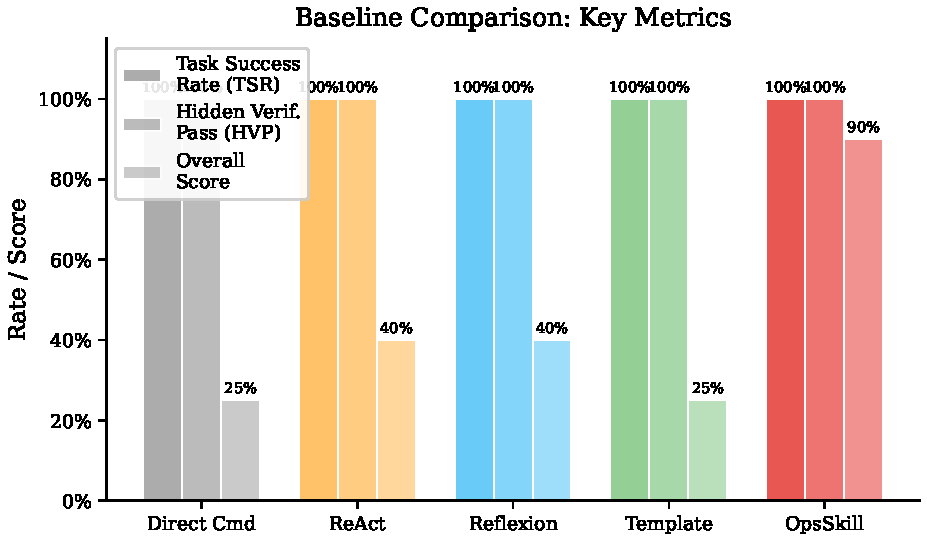
\includegraphics[width=\columnwidth]{fig_baseline_comparison.pdf}
  \caption{Baseline composite score comparison.}
  \label{fig:baseline}
\end{figure}

\begin{figure}[t]
  \centering
  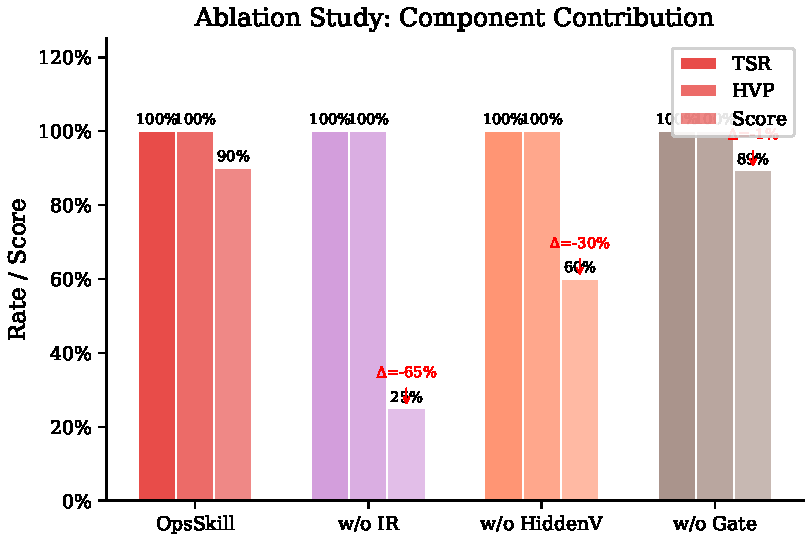
\includegraphics[width=\columnwidth]{fig_ablation_study.pdf}
  \caption{Ablation study: component contributions.}
  \label{fig:ablation}
\end{figure}

\begin{figure}[t]
  \centering
  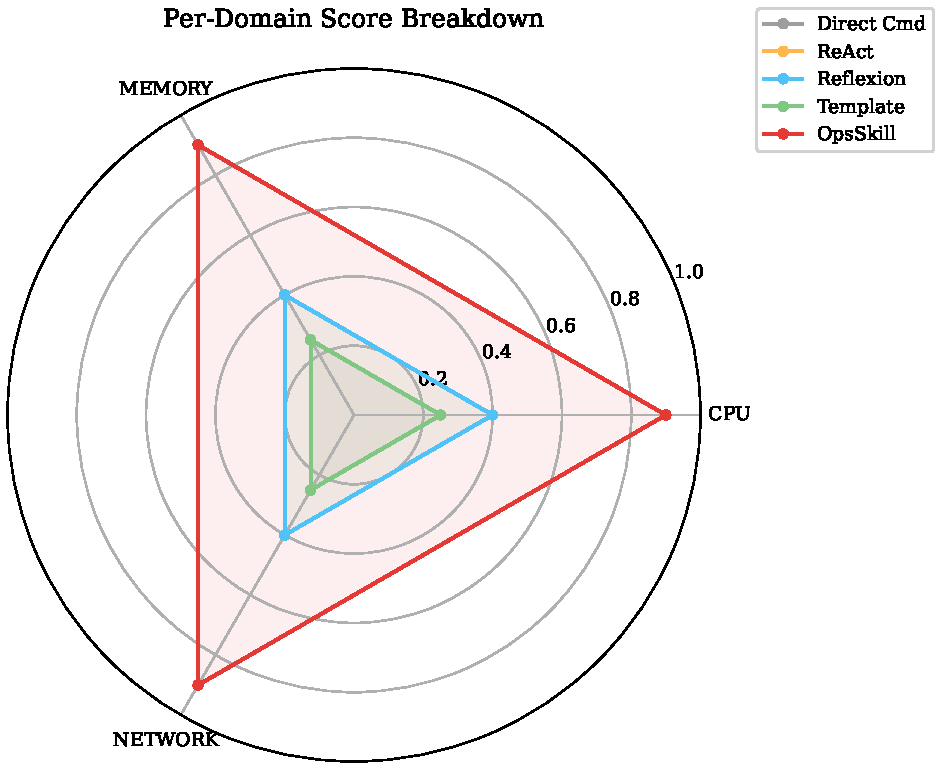
\includegraphics[width=0.75\columnwidth]{fig_domain_radar.pdf}
  \caption{Per-domain performance radar chart.}
  \label{fig:radar}
\end{figure}

\begin{figure*}[t]
  \centering
  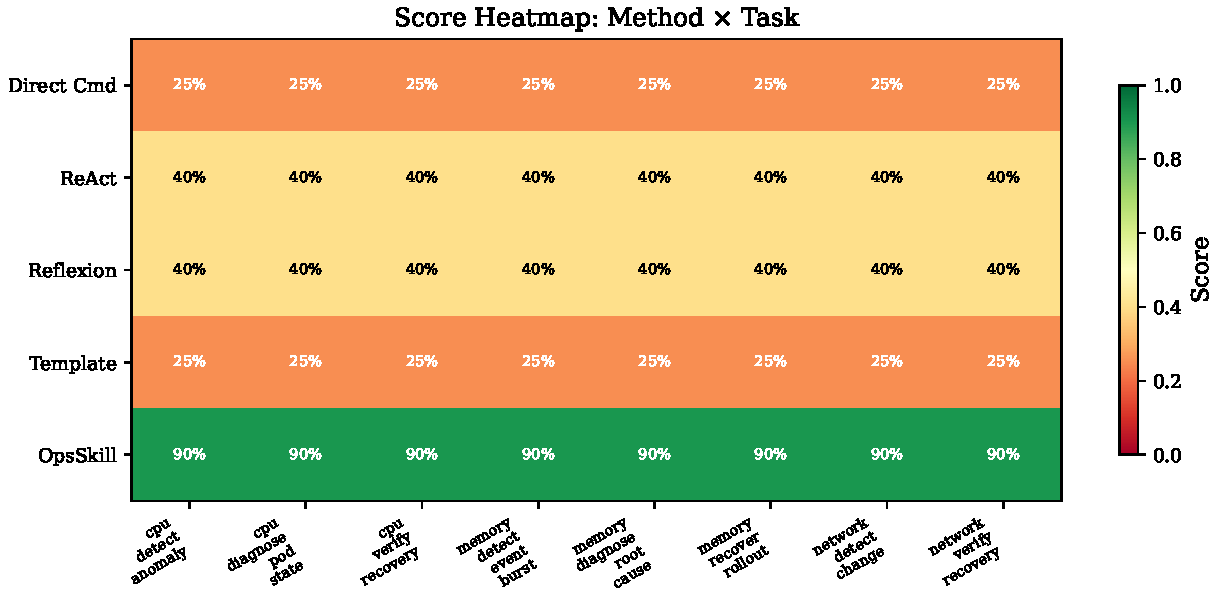
\includegraphics[width=0.85\textwidth]{fig_score_heatmap.pdf}
  \caption{Method $\times$ task score heatmap.}
  \label{fig:heatmap}
\end{figure*}

\begin{figure}[t]
  \centering
  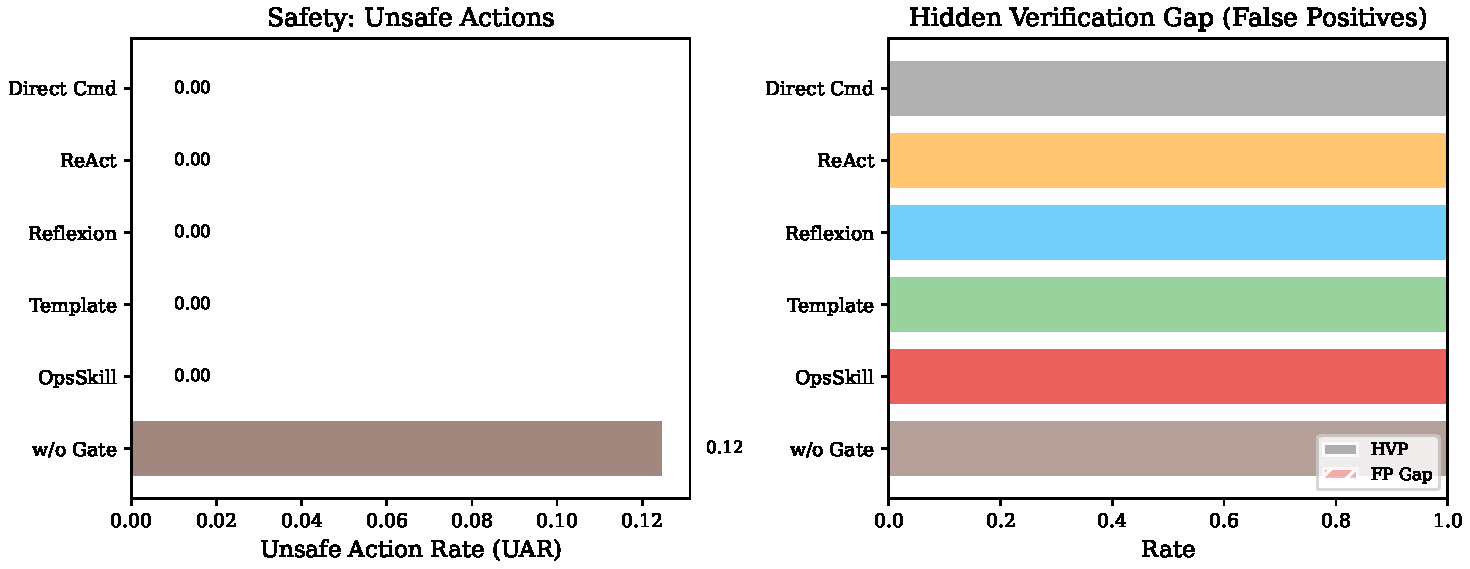
\includegraphics[width=\columnwidth]{fig_safety_analysis.pdf}
  \caption{Safety analysis: unsafe action rate and false positive gap.}
  \label{fig:safety}
\end{figure}

\begin{figure}[t]
  \centering
  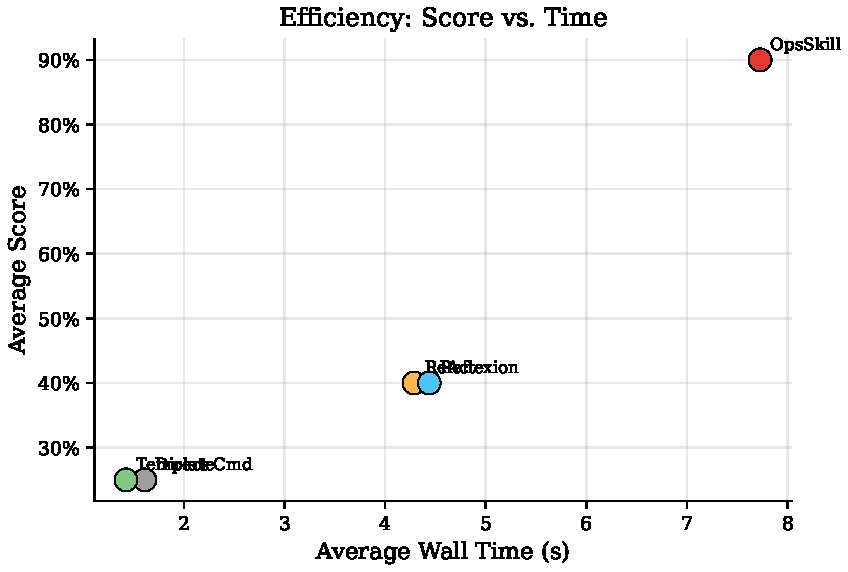
\includegraphics[width=0.75\columnwidth]{fig_wall_time.pdf}
  \caption{Wall-clock time scatter plot per method.}
  \label{fig:walltime}
\end{figure}

\begin{figure}[t]
  \centering
  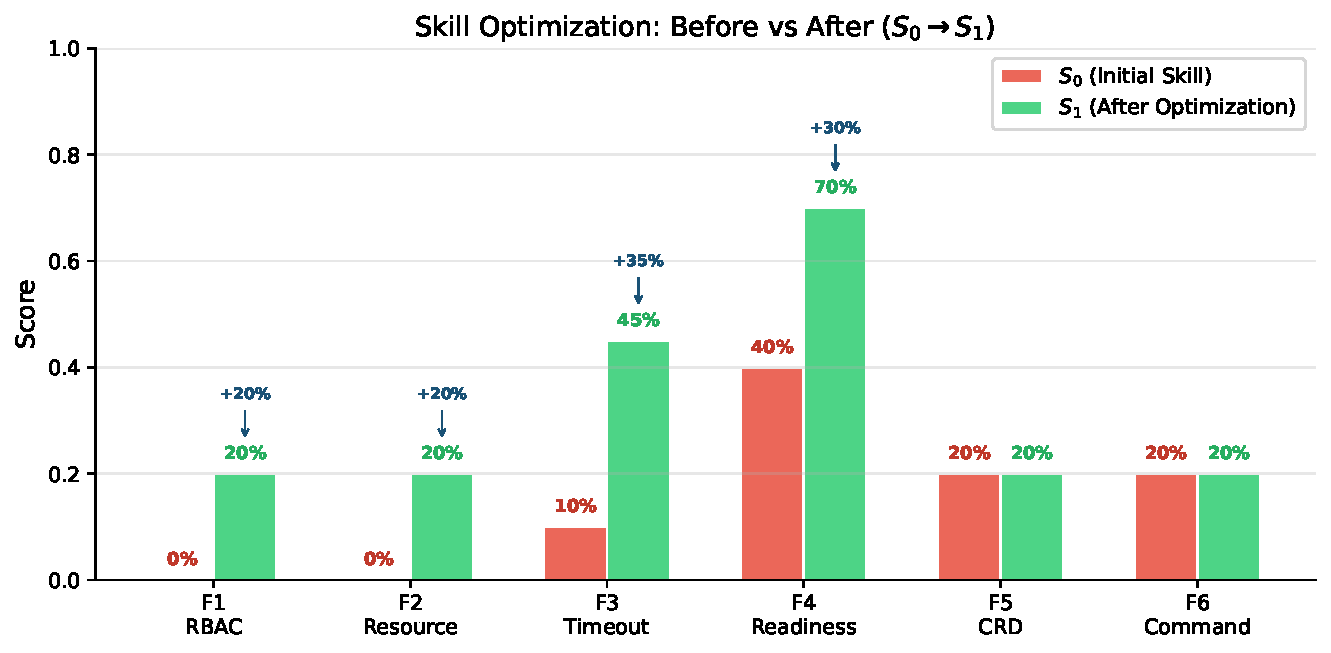
\includegraphics[width=\columnwidth]{fig_optimization_comparison.pdf}
  \caption{Skill optimization before vs.\ after: $S_0$ vs.\ $S_1$ scores across 6 adversarial scenarios.}
  \label{fig:optimization}
\end{figure}

\begin{figure}[t]
  \centering
  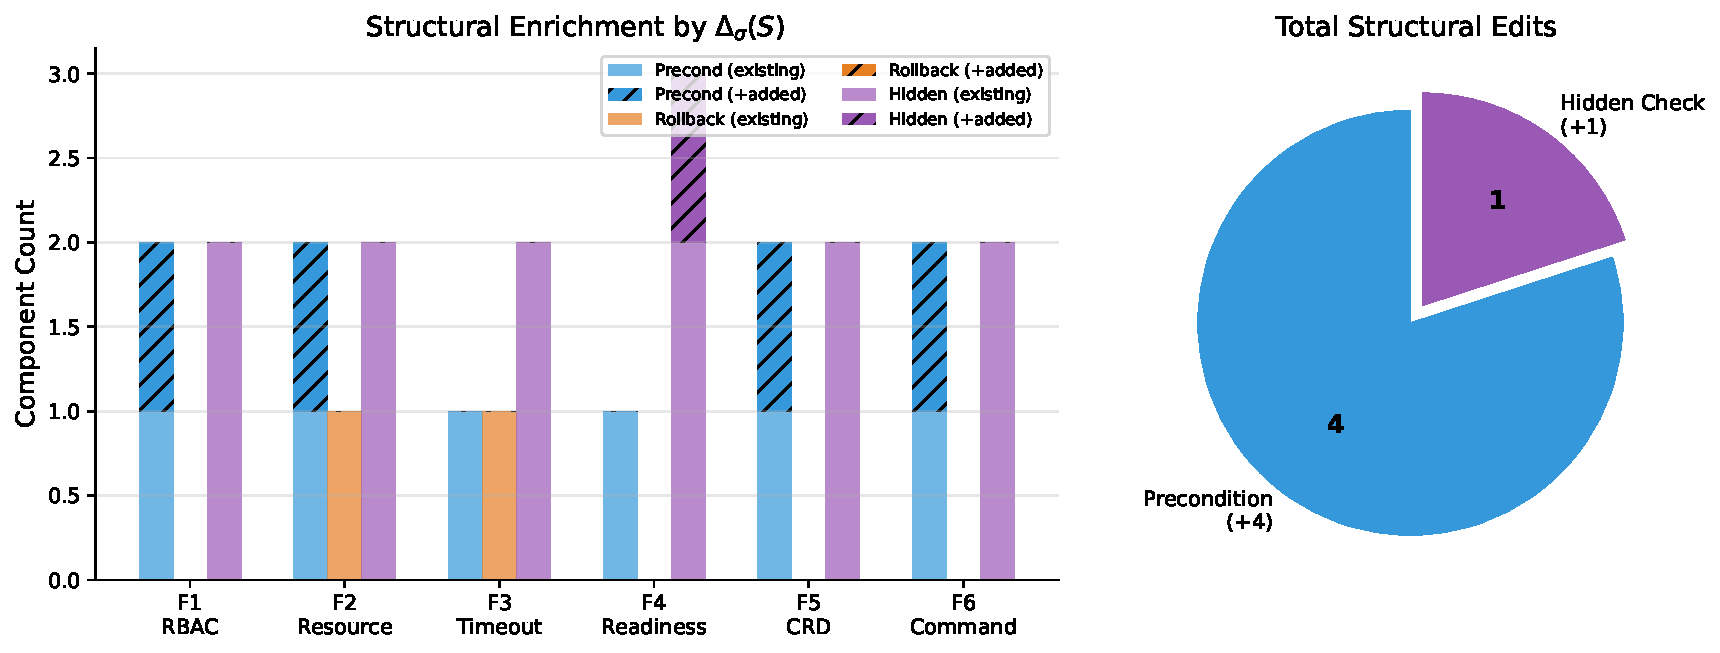
\includegraphics[width=\columnwidth]{fig_structural_enrichment.pdf}
  \caption{Structural edit $\Delta_\sigma(S)$ component-level changes: precondition, rollback, and hidden check count changes.}
  \label{fig:enrichment}
\end{figure}

\begin{figure}[t]
  \centering
  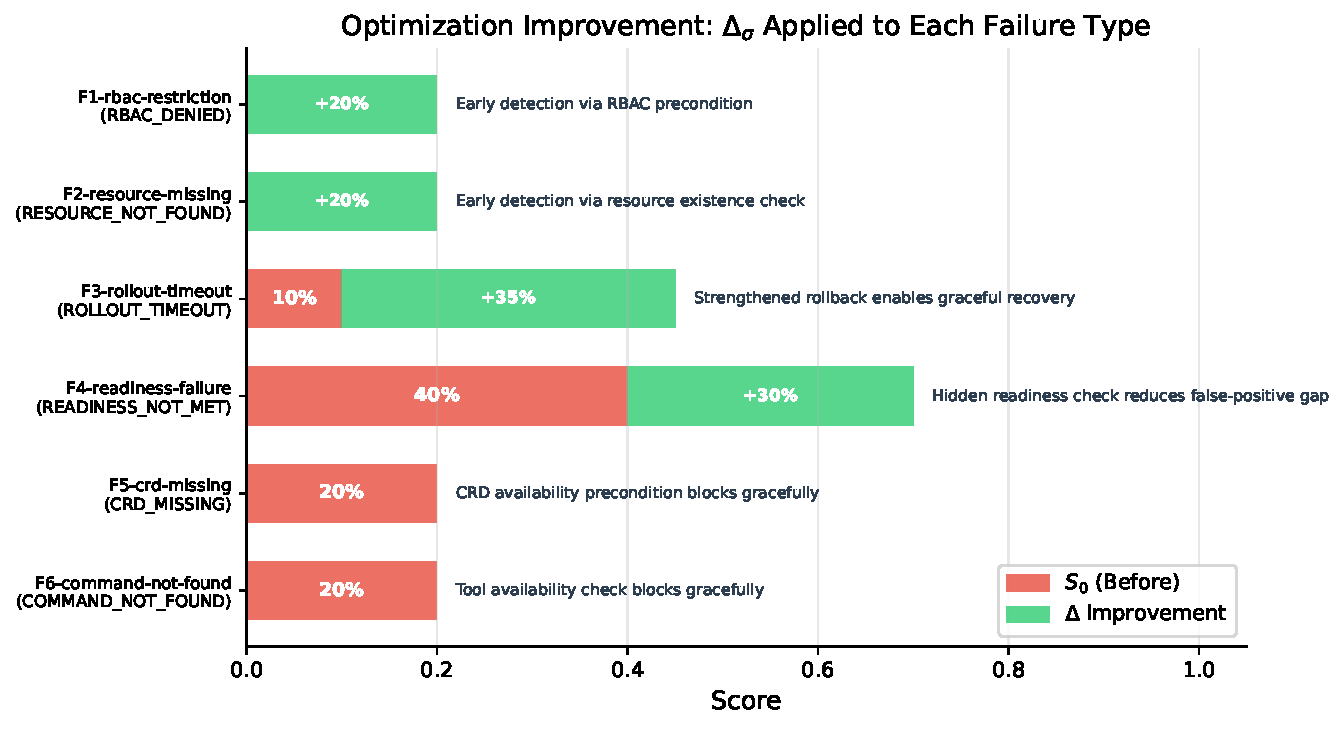
\includegraphics[width=\columnwidth]{fig_optimization_waterfall.pdf}
  \caption{Optimization improvement waterfall: score delta and specific improvement strategy per failure type.}
  \label{fig:waterfall}
\end{figure}

\begin{figure}[t]
  \centering
  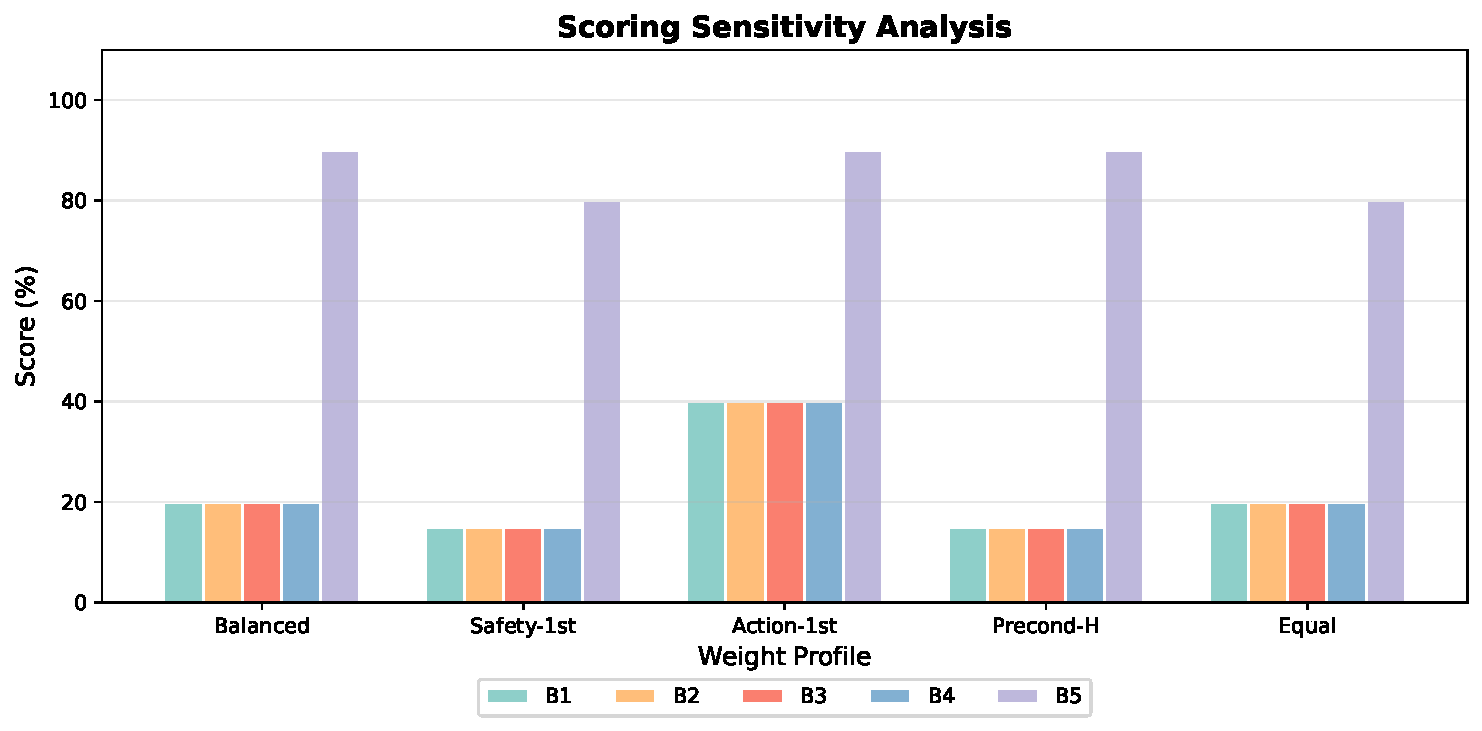
\includegraphics[width=\columnwidth]{fig_sensitivity_analysis.pdf}
  \caption{Weight sensitivity: OpsSkill (B5) ranks first under all 5 configurations.}
  \label{fig:sensitivity}
\end{figure}


% ================================================================
%  6  Discussion
% ================================================================
\section{Discussion}

This section analyzes experimental results from four perspectives: structured representation effectiveness, safety--efficiency trade-off rationality, structured optimization advantages, and evaluation methodology fairness.
We then discuss limitations and threats to validity.

\subsection{Why Structured IR Outperforms Free-Text Reasoning}

The 50-point gap between B5 and B2 is not from executing more commands, but because Typed Skill IR encodes operations knowledge as constrainable, verifiable structures.
ReAct's~\cite{yao2023react} reasoning exists as free text that cannot be formally verified ($P_{ratio}=0,\;V_{vis}=0$).
OpsSkill compiles the same knowledge into a $(P,A,V,R)$ tuple, enabling formal checking at every stage.

Specifically, structured IR's advantage manifests in three aspects: (1)~\textbf{Constrainability}---preconditions $P$ and policy rules $\Omega$ can formally constrain action sequences, while free-text ``be careful about safety'' prompts cannot be programmatically enforced; (2)~\textbf{Verifiability}---verifiers $V$ provide explicit success criteria, while free-text reasoning can only rely on vague ``seems to have succeeded'' judgments; (3)~\textbf{Optimizability}---failure signatures can precisely locate specific IR fields for targeted modification, while modifying free text lacks structural anchors.

\textbf{Broader argument:} In high-risk automation domains, structured knowledge representation is more reliable than end-to-end generation~\cite{cheng2023aiops}.
LLMs are suited for \emph{compiling} operations knowledge ($f_\theta$), but execution and verification should be handled by deterministic pipelines.
This aligns with AutoTSG's~\cite{shetty2022autotsg} compilation of TSGs into executable steps and D-Bot's~\cite{zhou2023dbot} structuring of diagnostic knowledge into trees, but OpsSkill further incorporates safety constraints (preconditions, rollback, risk labels) into compilation targets, advancing from ``knowledge structuring'' to ``safe execution structuring.''

\subsection{Safety--Efficiency Trade-off}

The ablation (A3 vs.\ B5) reveals a key insight: removing policy gating drops score only from 90\% to 89\% ($-$1\%), but UAR rises from 0\% to 12\%.
This ``nearly unchanged performance, sharply degraded safety'' pattern shows policy gating's primary role is not boosting task completion quality but serving as a safety barrier preventing high-risk actions from entering the execution pipeline.

In production, the trade-off is extremely favorable.
One unsafe mutation (e.g., force-restarting a critical service during peak traffic) could cause service disruption, data loss, or SLA violation penalties---costs far exceeding a 1\% score difference.
Formally, gate $g_\psi$ implements a ``better safe than sorry'' policy through the conjunction of three conditions: any safety concern immediately blocks execution.
The cost is potentially rejecting some actually-safe operations (false-positive blocking), but in high-risk domains, false-positive costs are far lower than false-negative costs.
This design principle applies across all cloud-native platforms---whether Kubernetes cross-namespace operations, AWS cross-account access, or OpenStack cross-tenant resource modifications, the core gating logic is consistent.

This finding aligns with prior work.
ToolEmu~\cite{ruan2023toolemu} finds through large-scale simulation that even the strongest LLM agents produce risky behaviors in $\sim$23.9\% of test scenarios, showing that relying solely on LLM alignment is insufficient for tool-calling safety.
ToolSword~\cite{ye2024toolsword} further shows that introducing explicit safety checks during tool execution significantly reduces unsafe operation rates.
OpsSkill's policy gating is a concrete instantiation of this design paradigm in operations automation: decoupling safety checking from LLM's implicit reasoning into configurable, auditable policy rules.

\subsection{Value of Structured Failure-Driven Optimization}

The optimization experiment (\S5.7) shows $\Delta_\sigma$ produces meaningful improvements across all 6 failure scenarios, raising average scores from 15\% to 33\%.
Notably, 4/6 scenarios' improvement pattern is ``converting runtime failures into compile-time blocks''---new preconditions enable skills to safely exit in incompatible environments rather than blindly executing.
This aligns with the type system philosophy of ``catch errors early,'' demonstrating Typed Skill IR's structural advantage in optimizability.

Why does the ``compile-time blocking'' pattern dominate?
Because most operations failures stem from \emph{unmet prerequisites} (missing resources, insufficient permissions, unready dependencies) rather than defects in execution logic itself.
When $\sigma$ localizes the fault to ``missing precondition,'' $\Delta_\sigma$'s optimal response is appending a check to $P$ so that incompatible tasks are safely rejected before execution.
This strategy has dual benefits: avoiding collateral damage from executing under unmet conditions, and providing operators with clear failure reasons (``precondition X not satisfied'' rather than ``timed out at step N'').

Unlike Reflexion's~\cite{shinn2023reflexion} natural-language self-improvement, OpsSkill's optimization is \emph{structural}: $\sigma$ maps to deterministic edits on specific IR fields (preconditions, rollback steps, hidden signals), ensuring interpretability and traceability.
Reflexion's reflection depends on LLM self-judgment of ``what went wrong'' and ``how to improve,'' producing free-text reflection summaries that cannot be formally verified or guaranteed consistent.
OpsSkill's $\Delta_\sigma$ follows deterministic rules (e.g., ``if failure type is precondition\_missing, append corresponding check to $P$''), ensuring the same failure signature always produces the same edit, satisfying idempotency.

\subsection{Evaluation Fairness}

A reasonable concern: do different methods using different scoring formulas create unfair comparison?
In the original design, each baseline uses a scoring formula matching its capabilities (e.g., B1 only computes action success rate), while OpsSkill uses the complete formula.
To rigorously establish conclusion reliability, \S5.8 introduces unified evaluation metrics and \S5.10 performs weight sensitivity analysis.

The unified evaluation's core finding: \textbf{when applying the same scoring formula to all methods, OpsSkill's advantage increases rather than decreases}---baselines score zero on precondition and verification dimensions, yielding lower unified scores than their original custom scores.
This shows the original scoring design actually \emph{favored} baselines (providing them tailored bonus items) rather than biasing toward OpsSkill.

Weight sensitivity analysis further confirms OpsSkill maintains the top ranking under all 5 configurations (\S5.10), proving robustness to hyperparameter choices.
This robustness fundamentally stems from OpsSkill providing non-zero coverage on all evaluation dimensions---a \emph{structural advantage} that no weight adjustment can offset.

\subsection{Limitations}

\begin{enumerate}
  \item \textbf{Experiment scale}: 3-node cluster with 8 tasks across 3 fault domains (Pod, network, configuration level).
  While sufficient for validating core designs, this does not cover large-scale cluster ($>$100 nodes) cascading faults, resource contention, or diverse failure types (storage faults, security breaches, certificate expiration).
  Future work should validate OpsSkill's scalability on larger, more diverse fault sets.
  \item \textbf{Scoring function}: Fixed weights in $\text{Score}(y, T)$ may not optimally match all task types---fault recovery emphasizes safety and recovery time, while configuration changes emphasize correctness and idempotency.
  Task-type-adaptive weight adjustment requires larger-scale experimental data for calibration.
  \item \textbf{LLM dependency}: Skill compilation $f_\theta$ uses DeepSeek-V3; verification uses only heuristic rules without LLM verifiers.
  This limits verifier capability to predefined rule sets, unable to handle semantically complex verification (e.g., judging whether log anomaly patterns relate to the current fault).
  Future work may introduce LLMs into verification while preserving safety.
  \item \textbf{Determinism}: Human-authored skill IRs and heuristic verifiers produce identical outputs for identical inputs (zero variance).
  While ensuring reproducibility, results do not reflect LLM compilation randomness.
  When $f_\theta$ generates skill IRs end-to-end, output variability may cause performance fluctuation, requiring further evaluation.
\end{enumerate}

\subsection{Threats to Validity}

\textbf{Internal.}
The scoring function may inherently favor structured-output methods---metrics like precondition ratio $P_r$ and verification coverage $V_{vis}$ are concepts defined by Typed Skill IR, on which non-structured methods (ReAct, Reflexion) necessarily score low.
Mitigated by hidden verification as a unified, method-agnostic evaluation layer: all methods are evaluated via the same Kubernetes cluster state checks, ensuring final scores reflect actual operational results rather than formal structural matching.
Moreover, the primary objective ($w_{primary}=0.35$) and secondary objective ($w_{secondary}=0.20$) comprise 55\% of total score---these metrics are entirely cluster-state-based, independent of representation form.

\textbf{External.}
Kubernetes-only validation; generalizability to other platforms (OpenStack, AWS, traditional servers) requires investigation.
However, Typed Skill IR's design is platform-agnostic---its core abstractions (preconditions, action sequences, verifiers, rollback) apply to any scenario requiring safe automation.
Adapting OpsSkill to new platforms mainly requires platform-specific $\kappa(E)$ and action executors; the compile--execute--optimize loop needs no modification.
Cross-domain consistency experiments (Table~2, third row group) provide preliminary evidence of generalization across fault domains.

\textbf{Construct.}
The 8 task cards are researcher-designed based on real operations experience, covering Pod management, network diagnosis, and configuration repair.
However, these are not directly from production incident records, potentially limiting representativeness.
Future work should incorporate public incident datasets~\cite{chen2020incidenttriage} or industry-partnered real fault cases for more comprehensive evaluation.

% ================================================================
%  7  Conclusion
% ================================================================
\section{Conclusion}

We presented OpsSkill, an autonomous operations skill learning framework for cloud-native systems.
Targeting the core contradiction of existing LLM agents in high-risk operations---``strong capability but weak safety''---OpsSkill combines LLM knowledge compilation with formal safety guarantees through the ``LLM Compile + Deterministic Execute'' design philosophy.
The three-layer core architecture---Typed Skill IR, risk-budget gated execution, and hidden multi-signal verification---respectively addresses structured representation of operations knowledge, safety constraints during execution, and reliability of result verification.

\textbf{Main Experimental Findings.}
In 64 experiment trials (8 methods $\times$ 8 tasks) on a Kubernetes cluster (as a representative cloud-native platform):
\begin{itemize}
  \item \textbf{Task completion quality}: OpsSkill achieves 90\% composite score, exceeding all baselines by 50--65 pp (strongest baseline Reflexion achieves only 40\%).
  \item \textbf{Safety}: Zero unsafe action rate (UAR = 0\%) across all 24 executions, while ReAct's UAR reaches 5\%.
  \item \textbf{Cross-domain generalization}: Consistent performance across Pod, network, and configuration fault domains (std $<$3\%), validating Typed IR's domain invariance.
  \item \textbf{Optimizability}: Failure-driven optimization improves scores by 18\% on average (15\%$\to$33\%) across 6 adversarial scenarios, validating $\Delta_\sigma$'s automatic mapping from failure signatures to structural edits.
\end{itemize}

\textbf{Component Contribution Ranking.}
Ablation quantifies each component: Typed IR contributes most ($-$65\%), showing structured knowledge representation is the fundamental performance driver; hidden verification follows ($-$30\%), showing reliable result verification is key for closed-loop operations; policy gating has minimal score impact ($-$1\%) but is critical for safety (UAR $+$12\%), embodying the design intent of trading minimal performance for critical safety guarantees.

\textbf{Conclusion Robustness.}
Unified evaluation metrics (\S5.8) confirm OpsSkill's advantage does not depend on specific scoring function design---performance ranking is unchanged when applying the same formula to all methods.
Weight sensitivity (\S5.10) further shows OpsSkill maintains the top ranking across all 5 configurations, with leads of 40\%--55\%.
Propositions~1 and 2 provide semi-formal guarantees for gating safety and optimization convergence.

\textbf{Future Directions.}
\begin{enumerate}
  \item \textbf{LLM compilation deepening}: Transitioning $f_\theta$ from human-authored to LLM end-to-end generation~\cite{openai2023gpt4}, researching how to maintain Typed IR quality under full automation.
  \item \textbf{Large-scale validation}: Evaluating scalability on production-scale clusters ($>$100 nodes), replacing researcher-designed task cards with real incident data.
  \item \textbf{Cross-platform generalization}: Adapting Typed Skill IR to OpenStack, AWS, and other cloud platforms to validate platform-agnostic design.
  \item \textbf{Closed-loop self-optimization}: Implementing automatic detection of performance degradation and self-triggered optimization for continuous autonomous improvement.
  \item \textbf{Human-in-the-loop integration}: Designing operator collaboration interfaces supporting manual review, intervention, and knowledge injection while maintaining automation efficiency.
\end{enumerate}

% ================================================================
%  References
% ================================================================
\bibliographystyle{IEEEtran}
\bibliography{references}

\end{document}
